%%=============================================
% !Mode:: "TeX:UTF-8"
% !TEX program  = XeLaTeX
%%=============================================
% 模板名称:hitszthesis
% 模板版本:V3.2.3
% 模板作者:杨敬轩(Jingxuan Yang)
% 联系作者:yangjx20@mails.tsinghua.edu.cn & yanglatex2e@gmail.com
% 模板交流:QQ群:1039392552,加群请备注LaTeX、hitszthesis相关说明
% 模板适用:哈尔滨工业大学(深圳)本、硕、博学位论文
% 模板编译:手动编译方法参看 README.md 或 hitszthesis.pdf
%          GNU make 工具:make thesis
%          Windows 批处理脚本:双击 compile.bat 自动编译论文
%          更多编译细节详见说明文档:hitszthesis.pdf
% 更新时间:2022/05/05
% 模板帮助:请**务必务必务必**阅读 hitszthesis.pdf 说明文档,文档查看方法:
%          cmd 命令行:texdoc hitszthesis
%          推荐前往模板的 GitHub 仓库获取最新文件,地址:
%          https://github.com/YangLaTeX/hitszthesis
%%=============================================

% 设置文档类别为 <hitszthesis>
% \documentclass[type=doctor]{hitszthesis}
% \documentclass[type=master]{hitszthesis}
\documentclass[type=bachelor,infoleft=true]{hitszthesis}

% 模板提供以下选项,各个选项之间不要有空格
% 1. type=bachelor|master|doctor
%   含义:本科、硕士、博士学位论文,不设默认值,**必填**
% 2. covertitletworow=true|false
%   含义:本科封面第一页标题单行或多行显示,默认为单行显示(false)
% 3. infoleft=true|false
%   含义:本科封面第二页下划线内容居中或居左显示,默认为居中显示(false)
% 4. mathfont=newtxmath|mtprotwolite|mtprotwo
%   含义:正文数学字体选项:newtxmath(默认),mtprotwolite(lite版,免费),
%         mtprotwo(完全版,需购买授权),
%         mtpro2字体官网:https://www.pctex.com/mtpro2.html
% 5. boldcaption=true|false
%   含义:图表题注是否加粗,默认为不加粗(false)
% 6. tocfour=true|false
%   含义:是否添加第四级目录,只对本科文科个别要求四级目录有效,默认不添加(false)
% 7. fulltime=true|false
%   含义:是否全日制,非全日制如同等学力等,要在coverinformation中设置类型,
%        默认是全日制(true)
% 8. subtitle=true|false
%   含义:论文题目是否含有副标题,默认没有副标题(false)
% 9. openright=true|false
%   含义:博士论文是否要求章节首页必须在奇数页,默认否(false)
% 10. library=true|false
%   含义:是否为提交到图书馆的电子版,默认否(false)
% 11. alphappendix=true|false
%   含义:本科毕业设计附录章节编号是否为大写字母,默认是(true)

% 自定义设置与额外加载的宏包请写在 \file{hitszthesis.sty} 里
\usepackage{hitszthesis}

% 图片存放路径,在这些文件夹里的图片可以直接使用图片文件名调用
\graphicspath{{figures/}{pictures/}}

\makeatletter
\newenvironment{breakablealgorithm}
  {% \begin{breakablealgorithm}
   \begin{center}
     \refstepcounter{algorithm}% New algorithm
     \hrule height.8pt depth0pt \kern2pt% \@fs@pre for \@fs@ruled
     \renewcommand{\caption}[2][\relax]{% Make a new \caption
       {\raggedright\textbf{\ALG@name~\thealgorithm} ##2\par}%
       \ifx\relax##1\relax % #1 is \relax
         \addcontentsline{loa}{algorithm}{\protect\numberline{\thealgorithm}##2}%
       \else % #1 is not \relax
         \addcontentsline{loa}{algorithm}{\protect\numberline{\thealgorithm}##1}%
       \fi
       \kern2pt\hrule\kern2pt
     }
  }{% \end{breakablealgorithm}
     \kern2pt\hrule\relax% \@fs@post for \@fs@ruled
   \end{center}
  }
\makeatother

%%=============================================
% 开始写论文
% !!注意本文仅作为排版格式示例,并不作为毕业论文规范
\begin{document}

% 若题目过长,则需使用以下命令调整本科封面第二页下划线长度
\infowidth = 9cm

% 开始写前言部分
\frontmatter

% 封面信息填写
% !TEX root = ../main.tex

\hitszsetup{
  %******************************
  % 注意:
  %   1. 配置里面不要出现空行
  %   2. 不需要的配置信息可以删除
  %******************************
  %
  %=====
  % 秘级
  %=====
  statesecrets={公开},
  natclassifiedindex={TM301.2},
  intclassifiedindex={62-5},
  %
  %=========
  % 中文信息
  %=========
  ctitleone={带时间敏感性的无人机网络},%本科生封面使用
  ctitletwo={扫描覆盖算法设计与实现},%本科生封面使用
  ctitlecover={带时间敏感性的无人机网络\\扫描覆盖算法设计与实现},%放在封面中使用,自由断行
  ctitle={带时间敏感性的无人机网络扫描覆盖算法设计与实现},%放在原创性声明中使用
  % csubtitle={一条副标题}, %一般情况没有,可以注释掉
  cxueke={工学},
  cpostgraduatetype={学术},
  csubject={计算机科学与技术},
  % csubject={机械工程},
  caffil={计算机科学与技术学院},
  % caffil={哈尔滨工业大学(深圳)},
  cauthor={胡聪},
  csupervisor={堵宏伟\enspace 副教授},
  % cassosupervisor={某某某 教授}, % 副指导老师
  % ccosupervisor={某某某 教授}, % 联合指导老师
  % 日期自动使用当前时间,若需指定按如下方式修改:
  cdate={2022年6月},
  % 指定第二页封面的日期,即答辩日期
  cdatesecond={2022年06月09日},
  cstudentid={180110505},
  % cstudenttype={同等学力人员}, %非全日制教育申请学位者
  %(同等学力人员)、(工程硕士)、(工商管理硕士)、
  %(高级管理人员工商管理硕士)、(公共管理硕士)、(中职教师)、(高校教师)等
  %
  %
  %=========
  % 英文信息
  %=========
  etitle={Research on robot intelligent grasping based on Neural Network},
  esubtitle={This is the sub title},
  exueke={Engineering},
  esubject={Mechanical Engineering},
  eaffil={Harbin Institute of Technology, Shenzhen},
  eauthor={Jingxuan Yang},
  esupervisor={Prof. XXX},
  % eassosupervisor={XXX},
  % 日期自动生成,若需指定按如下方式修改:
  edate={June, 2020},
  estudenttype={Master of Engineering},
  %
  % 关键词用“英文逗号”分割
  ckeywords={无线传感器网络, 无人机, 扫描覆盖, 贪心算法, 遗传算法},
  ekeywords={WSN, UAV, sweep coverage, greedy algorithm, genetic algorithm},
}

% 中文摘要
\begin{cabstract}

  近年来,随着无人机技术的高速发展,其在航拍、物流、农业、公共安全和救援等领域有着非常广阔的发展前景,在这些领域中,常常需要多架无人机对特定区域进行扫描覆盖任务。
  由于无人机的路线规划方案对无人机的扫描覆盖率有着较大的影响,因此针对无人机的路径优化研究就显得非常必要和有意义。


  本文根据国内外研究现状,以灾害发生后的应急救灾场景作为背景,着重考虑了无人机的特点和救援任务对时间的要求等因素,
  构建了多目标带时间窗的无人机扫描覆盖路径问题模型,以实现扫描覆盖率高和成本较低等多个目标。
  接下来分别采用贪心算法和遗传算法对该模型进行求解,最后通过结果分析验证了模型和算法的有效性。


\end{cabstract}

% 英文摘要
\begin{eabstract}

  In recent years, with the rapid development of unmanned aerial vehicle technology,
   it has a very broad development prospects in the areas of aerial photography, logistics, 
   agriculture, public safety and rescue, in which multiple unmanned aerial vehicles are often required to scan and cover specific areas. 
   Because the UAV's route planning scheme has a large impact on the UAV's scan coverage, it is necessary and meaningful to study the UAV's route optimization.

  
  In this paper, based on the research status at home and abroad, taking the emergency relief scenario after a disaster as the background, 
  and considering the characteristics of unmanned aerial vehicles and the time requirements of rescue tasks, 
  a multi-objective model of unmanned aerial scanning coverage path problem with time windows is constructed to achieve multiple goals such as high scan coverage and low cost. 
  Next, the greedy algorithm and genetic algorithm are used to solve the model. Finally, the validity of the model and the algorithm is verified by the result analysis.

\end{eabstract}


% 生成封面、中英文摘要
\makecover

% 物理量名称表,若采用标准符号则不需要此表
% % !TEX root = ../main.tex

% 物理量符号表,如果采用标准符号则不需要此表
\begin{denotation}
  % 此处最好是h
  \begin{table}[h]
  \caption{国际单位制中具有专门名称的导出单位}
  \vspace{0.5em}\centering\wuhao
  \begin{tabular}{ccccc}
    \toprule[1.5pt]
    量的名称&单位名称&单位符号&其它表示实例\\
    \midrule[1pt]
    频率&赫[兹]&Hz&s-1\\
    \bottomrule[1.5pt]
    \end{tabular}
  \end{table}
\end{denotation}


% 中文目录
\tableofcontents

% 英文目录,本硕不要求
% \tableofengcontents

% 开始写正文
\mainmatter

% 第1章
% !TEX root = ../main.tex

% 中英标题:\chapter{中文标题}[英文标题]
\chapter{绪论}[Introduction]

\section{课题背景及研究的目的和意义}[Background, objective and significance of the subject]

% 正文内容,注意LaTeX分段有两种方法,直接空一行或者使用<\par>
% 默认首行缩进,不需要在代码编辑区手动敲空格
我国的自然灾害发生较为频繁,带来了严重的社会危害。据统计,中国是世界上自然灾害发生频率最高,且造成后果最严重的的少数几个国家之一\cite{ziranzaihaifangzhide}。中国的自然灾害种类多,发生频率较高,且灾情十分严重。
在自然灾害产生后,首要任务是进行救援和救灾。在重大自然灾害发生后,不仅会给社会经济造成较大的损失,更严重的情况下可能会造成受灾地区通信中断和物资供应中断,甚至导致威胁人身安全。研究表明,
自然灾害发生后的黄金救援期为72小时,而灾区需要的物资多为紧急需要的医疗物资和生活物资等,因此顺利且准时地将救援物资投放到受灾地区成为了衡量救灾任务是否成功的决定性因素之一。\cite{yuqingqing}
高效且准确的应急救援行动可以提高物资的运输效率,同时减少救援所需要的时间,从而有效降低自然灾害造成的损失,保护人民群众的生命财产安全。


自然灾害的发生属于突发性事件,是难以避免的,但是通过对应急救援场景的分析,从而确定符合实际需求的应急救援物资调度方案,可以确保救援工作的高效进行和救援物资的及时合理分配。
无人机(Unmanned Aerial Vehicle,UAV)作为无人驾驶飞行器,具有实时性强、不容易受外界环境影响、部署条件较为灵活和使用维护成本较为低廉等特点。
突发事件的种类具有多样性,灾区现场的复杂环境导致与人工救援相比,使用无人机进行救援工作有着较大的优势。采用无人机代替人工作业,能够有效减少意外事故风险,同时能够节省人力资源。
目前,我国的无人机工业发展迅速,载重无人机在救援救灾领域中已得到较为广泛的应用。在货运车辆受限于环境无法抵达灾区时,载重无人机就能替代货运车辆,起到救援物资投放的作用。\cite{liuyajing}


在确定了使用无人机进行救援工作后,我们需要对无人机调度和救灾任务进行合理的规划,以满足救援工作的实习需求。在无人机数量和救援地点数量的影响之下,救援任务的分配也变得较为复杂。
随着无人机协同工作技术的发展,救灾的前期准备工作时间得以大幅较少,从而使得救灾任务的效率得到提升。


本文以灾区环境下针对突发自然灾害的多无人机协同调度救灾问题为背景开展研究,建立带时间敏感性的无人机网络扫描覆盖问题的模型,研究目标是在满足各灾区救援点时间敏感和无人机的载重上限条件下,
如何尽可能地提高无人机对灾区救援行动的扫描覆盖率,同时使得救援成本尽可能维持在较低水平。


\section{国内外研究现状}[Current research state]

\subsection{无人机在应急救灾方面的应用}[Application of UAV in emergency relief]
2008年,国产千里眼无人机对四川汶川大地震后的北川县城进行了拍摄,成为了抗震救灾过程中的重要参考资料。此后,近年来随着新兴科技成果的迅速转化和对灾害救援要求的不断提高,无人机在防灾、减灾和救灾领域的应用越来越频繁和多样。
凭借着无人机的高灵活性和高机动型,其在应急救灾领域始终发挥着重要的作用。目前,国内外已有不少企业将目光投向无人机技术。在2013年,Amazon就开始尝试使用无人机进行物流配送,并且Amazon推出了新型混合动力物流无人机Prime Air Drone,该款无人机支持垂直起降,
续航里程可达30公里,除此之外Amazon还为其开发了计算机视觉识别技术,可以使无人机自动寻找合适的降落点。\cite{zhanghonghai}而在国内企业中,顺丰速运和京东作为物流行业中的领军企业,均较早提出了无人机用于物流和救灾方面的构想。顺丰主张主线路高容量运载自动驾驶飞机、分支线路中运载量自动驾驶飞机和末端物资配送自动驾驶飞机结合的三段式空运网络。目前,无人机应急救灾和配送的研究已经十分成熟。将无人机应用到应急救灾领域中,可以充分配合其他工具,从而实现“1+1>2”的效果。在2020年初新型冠状病毒感染的肺炎疫情期间,顺丰速运在武汉市、温州市和哈尔滨市等地投入了大量无人机,主要负责运送
防护服、口罩、手套、生活物资、药品等继续的救援物资,其在上述城市的单日运送总量达到1.8吨,飞行总里程超过1500公里。顺丰速运表示,顺丰的无人机主要用途是将货物运送至较难进行配送覆盖的偏远地区,这与将无人机应用于应急救灾领域的构想不谋而合。2020年,京东也推出了自主研发的物流无人机,载重可高达数百公斤,可用于应急救援时的大规模物资运输投放,提高救援效率。\cite{renxuan}


下表是部分物流无人机的参数信息。
  \begin{table}[htbp]
    \vspace{0.5em}\centering\wuhao
    \caption{部分物流无人机参数}
    \begin{tabular}{cccc}
    \toprule[1.5pt]
    公司 & 型号 & 最大载重 & 最大续航里程 \\
    \midrule[1.5pt]
    亚马逊 & Prime Air Drone & 2.5kg & 30km \\
    顺丰 & Ark & 12kg & 20km \\
    顺丰 & Manta Ray & 10kg & 100km \\
    京东 & 京蜓 & 数百千克 & 未公布 \\ 
    \bottomrule[1.5pt]
    \end{tabular}
    \end{table}

\subsection{无人机的路径规划问题研究现状}[Research state of UAV routing problems]
扫描覆盖作为无线传感器网络(Wireless Sensor Networks, WSN)的一个新兴领域,近年来收到了广泛的关注。通常情况下,根据问题的最终优化目标,扫描覆盖问题可分为以下三个类型:
\begin{itemize}
  \item [(1)] 传感器数量的优化。这类问题的目标是最小化区域内扫描覆盖范围的移动传感器数量。解决这类问题的一般出发点是较少移动传感器在目标区域内的移动距离。
  Cheng等人在文献中证明,解决该问题的算法是NP-Hard的,并据此提出了一种称为CSWEEP的启发式算法\cite{2008Sweep};
  \item [(2)] 扫描覆盖时间周期的优化。该问题的目标是最小化对区域内所有兴趣点进行扫描覆盖所投入的时间。Feng等人在文献中提出了目标是最小化扫描覆盖总时间(M$^3$SR)的问题\cite{2015Shorten};
  \item [(3)] 传感器传输延迟的优化。该问题的目标是降低数据中心与移动传感器通信过程中的通信延迟,Zhao等人在文献中提出了有啊传感器延迟的解决方案\cite{2012zhao}。
\end{itemize}


与上述研究领域的目标不同,本文主要研究的是无人机的路径规划问题。其与车辆路径规划问题(Vehicle Routing Problem, VRP)较为相似,因此在研究时可以参考车辆路径问题领域的相关方法。
在历来的研究中,使用同一型号车辆的车辆调度问题认为是旅行商问题(Traveling Salesman Problem, TSP)的特殊情况\cite{bektas2006multiple}。同时研究表明,该问题是一个NP-hard问题\cite{lenstra1981complexity}。


随着车辆路径规划问题在实际应用过程中的不断发展,其又产生了许多不同目标和不同领域的扩展,包括多型号车辆的车辆路径规划问题\cite{pan2021multi}、随机需求的车辆路径规划问题\cite{saint2021time}、单一车辆多次投入使用的车辆路径规划问题\cite{euchi2021hybrid}和带收集的车辆路径规划问题\cite{fan2021time}等。
而本文中所涉及的车辆路径规划问题被称为带时间窗的车辆路径规划问题(Vehicle Routing Problems With Time Windows, VRPTW)。在带时间窗的车辆路径规划问题中,兴趣点拥有时间窗限制,车辆需要在时间窗内访问兴趣点,并找到对兴趣点实现最大准时覆盖率的路径\cite{ren2022vehicle}。


对于NP-hard问题,使用精确算法进行求解并不现实,因此目前解决VRPTW问题的主要方法为启发式方法。较为简单的启发式方法的代表类型是贪心算法,在使用贪心算法求解问题时一般选择当前最优解,而非考虑整体情况的最优解,其较为简单,且拥有求解速度快的优点,但是只适合求解问题规模较小的NP-hard问题。
而智能优化算法主要包括模拟退火算法(Simulated Annealing, SA)、蚁群算法(Ant Colony Optimization, ACO)、禁忌搜索算法(Tabu Search, TS)和遗传算法(Genetic Algorithm,GA)等。模拟退火算法能够快速收敛,是一种全局搜索算法\cite{lee2021simulated}。蚁群算法根据蚂蚁的觅食行为进行设计,蚂蚁的觅食路径就是优化问题的解决方案。
蚁群内的蚂蚁可以通过某种信息机制实现信息的传递,其会在其经过的路径上释放一种可以称之为“信息素”的物质,蚁群会沿着“信息素”浓度较高路径行走,在正反馈机制下,蚁群会集中在信息素浓度较大的路径上,从而得到了问题的最优解\cite{wu2021hybrid}。禁忌搜索算法最先被Willard等人应用到车辆路径规划问题中\cite{ilhan2021improved},属于局部搜索算法。遗传算法根据大自然中生物的进化规律设计,模拟了达尔文生物进化论中的自然选择和遗传学中的生物进化过程,在求解较复杂的组合优化问题时,能较快地获得较好的优化结果。


而带时间窗的无人机路径规划问题(Unmanned Aerial Vehicle Routing Problems With Time Windows, UAVRPTW)作为带时间窗的车辆路径规划问题的变种,目前也在持续发展中。Choi等人在文献中提出了一种针对无人机续航有限问题的新型路径规划问题,他们将无人机的扫描覆盖任务定义为起飞、巡航、悬停、转弯和着陆五个阶段,并且提出了新的路径优化模型\cite{2019Energy}。Li等人在文献中提出了无人机的最短时间最大覆盖问题(MTMC),即在无人机性能的约束下,
在给定的区域内,实现在最短的时间内对兴趣点实现最大覆盖的目标,他们考虑了无人机的性能,并进行了数学建模,将多目标优化问题转化为单目标路径规划问题,取得了较好的优化结果\cite{2020A}。Thibbotuwawa等人在文献中提出了带无人机充电中心的UAVRPTW数学模型和算法,解决了无人机飞行的局限性\cite{thibbotuwawa2020unmanned}。


然而,过往的研究中大多忽视了无人机的返回时间,且较少考虑无人机的载重问题与传统载重车辆存在较大差异,本文对此问题作出了改进,确保了无人机能够在续航时间结束前返回基地,并考虑了无人机的最大载重问题。
\section{本文的主要研究内容}[Main research contents of this subject]

本课题的主要研究目标是解决带时间窗的无人机扫描覆盖路径规划问题并根据问题的解决算法设计出一套无人机紧急救援模拟系统。

本文的主要工作包括:
\begin{itemize}
  \item [(1)] 
  带时间敏感性的无人机网络扫描覆盖问题的建立。


  首先针对应急救援过程中的关键要素,如无人机基地、兴趣点、无人机等进行分析,然后需要分析无人机进行应急救援的全部流程,找到提高无人机飞行效率的方法和解决问题的整体流程。
  针对无人机应急救援问题,结合无人机自身的物理特性约束,建立了单目标的无人机应急救援问题模型,并针对该模型进行了参数的假设。在此基础上,设计了模型的数学表达式和问题的优化目标。
  \item [(2)]
  带时间敏感性的无人机网络扫描覆盖问题的算法设计。


  根据问题模型,设计了问题解的表达方式和初始解的产生方法。本文主要采用两种启发式算法——带载重的贪婪成本选择算法和带自交的遗传算法进行实验和求解。
  \item [(3)]
  算法性能的评估与对比。


  根据对实际场景的分析,设置了问题模拟中的场景参数和算法参数,对模型进行求解。得到结果后,还需要对实验结果进行分析,主要需要分析几种算法的可行性和性能优劣,验证通过改进后的算法能否得到求解问题模型的预期结果。
  \item [(4)]
  无人机紧急救援系统的模拟实现。


  在得到问题求解算法后,需要基于该算法为原型,进行相应的技术选型,并分析任务目标和任务需求,设计系统的总体框架和各模块功能,并对系统进行模拟实现。
\end{itemize}

% 第2章
% !TEX root = ../main.tex

% 中英标题:\chapter{中文标题}[英文标题]
\chapter{无人机紧急救援系统分析及问题模型构建}[Analysis and Problem Model Construction of UAV Emergency Rescue System]

\section{问题分析}[Problem analysis]
无人机是本课题中所涉及的紧急救援系统的主体,因此在将无人机应用于紧急救援和物资投放时,要综合分析无人机的特点,
在考虑其优势的同时,也要分析其劣势对于救援系统的影响,并在系统设计中做到扬长避短,充分利用无人机本身的特性。


经过综合分析,我们发现无人机在紧急救援系统中,具有以下特点:
\begin{itemize}
	\item [(1)] 
	无人机的续航能力制约了其飞行距离


	\qquad 目前,大多数无人机均采用电池驱动,受制于目前的电池技术发展,民用货运无人机最大历程约为300km,
	且在载重情况下飞行,无人机的续航时间将会进一步降低,同时无人机在电量不足时还需要返回调度中心进行充电\cite{jin2017}。
	\item [(2)]
	无人机相较于大型物资供应车辆,行动更加灵活


	\qquad 自然灾害发生后,受灾地区往往会面临道路中断和交通阻塞等困难。如果使用传统大型物资供应车辆供应物资,
	很有可能会导致紧急物资供应不及时。而无人机在飞行至一定高度后,其行动路径将不会受到上述问题的阻碍,理论上
	可以进行点到点的直接飞行,有效提高了应急救援物资的配送效率\cite{chenhao2019}。
	\item [(3)]
	无人机的飞行受我国法律限制


	\qquad 目前,我国一些地方对于无人机的飞行管理十分严格,设立了禁飞区和管控区等\cite{shu2020},这导致我们在设计无人机紧
	急救援系统时,应该结合实际情况,有效避免无人机的飞行轨迹经过禁飞区。
	\item [(4)]
	民用无人机的载重能力有限


	\qquad 随着无人机技术的不断发展,目前无人机的载重能力已经有了大幅的提升。但是目前重载无人机多用于军事领域,
	在民用领域鲜有使用。因此在设计无人机紧急救援系统时,无人机负责进行的配送物资多为紧急需要的医疗物资和部分
	较轻的生活物资等,在使用无人机进行物资配送时需要考虑这一特点\cite{liuping2016}。
\end{itemize}

\section{带时间敏感性的无人机网络扫描覆盖问题的建立}[Establishment of Scanning Coverage Problem for UAV Networks with Time Sensitivity]

本课题中提出的无人机紧急救援系统,主要包含了无人机基地、救援点和无人机等,同时还包括无人机调度的优化目标、
约束条件以及求解模型所对应的算法等。该紧急救援系统的总体设计如\figref{fg201}所示:

\begin{figure}[ht]
	\centering
	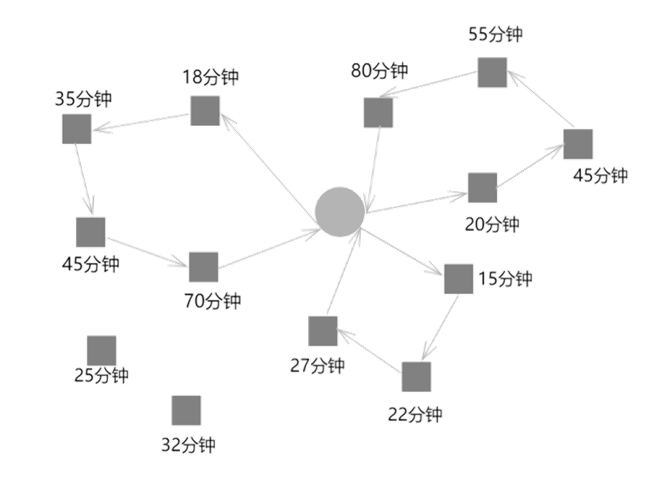
\includegraphics[width = 0.6\textwidth]{fg1_timesensitive}
	\caption{无人机紧急救援系统}
	\label{fg201}
\end{figure}

\begin{itemize}
	\item [(1)]  
	无人机基地和物资仓库(以下简称“基地”)


	\qquad 基地在紧急救援系统中主要负责救援物资的仓储、无人机的调度和无人机的维护充电等工作。当救援物资从
	上游运送到基地后,其能够根据灾区目前的受灾情况和无人机状态等信息,计算和生成无人机调度方案。同时,基地
	也负责对返回基地的无人机进行维护和充电等工作,也是无人机进行起飞和降落的起点和终点。

	\item[(2)]
	救援物资

	
	\qquad 在无人机救援过程中,需要考虑救援物资的质量、大小和配送终点等。在救援物资上印有唯一的身份信息标识,
	基地中的扫描系统可以通过该身份信息标识获取该批救援物资的全部信息,并将这些信息存放在基地的信息管理系统中。

	\item[(3)]
	无人机

	
	\qquad 无人机是课题中紧急救援系统的核心。在无人机执行救援任务时,要对无人机的型号、续航里程、巡航速度和
	最大载重等特性进行研究。民用无人机多用电池续航,采用北斗或GPS导航进行定位,附带有摄像头,可以对救援地点
	进行航拍,以便基地了解受灾地点的现场情况。

	\item[(4)]
	待救援地点


	\qquad 在救灾过程中,无人机需要在一定时间内快速到达需要被救援的地点,以提供支援。这些地点对于时间要求较为敏感,
	如果无人机不能及时到达,可能会错过最佳救援时机,我们称这些点为兴趣点(Point of Interest,POI)。如\figref{fg201}所示,每个兴趣点都会
	有不同的时间敏感性,如果兴趣点的时间敏感性为15分钟,这意味着这个兴趣点需要在15分钟内被无人机所覆盖。

	\item[(5)]
	问题的优化目标

	\qquad 为了切实保障人民群众生命财产安全,在规划无人机的飞行路径时,应该以实现对更多兴趣点的有效覆盖作为首要目标。
	在实现以上目标的基础上,还需要考虑无人机的调度总成本和飞行距离等因素。在参考了大量有时间窗车辆路径问题
	(Vehicle Routing Problems With Time Windows,VRPTW)后,把主要的优化函数目标概括为:有效覆盖率和准时覆盖率最大化、
	救援成本最小化和无人机的飞行里程最小化,同时满足无人机不超重运输的目标。

	\item[(6)]
	约束条件
	

	\qquad 在VRPTW问题中,需要考虑车辆的载重、运输时间窗和运输完成后车辆必须返回基地等。而当VRPTW问题的主体变为无人机后,
	还需要考虑无人机的续航里程等无人机特有的约束条件。

	\item[(7)]
	问题的求解算法


	\qquad 本文在求解该问题时主要研究了两种算法,一种是改进的贪心算法,另一种是改进的遗传算法。在面对简单问题时,贪心算法
	简单且得到解的速度较快,但当问题较为复杂时,遗传算法是解决该问题的较好选择。
\end{itemize}

\section{无人机紧急救援系统的主要工作流程}[Main workflow of UAV emergency rescue system]
紧急救援系统的主要工作流程如\figref{fg202}所示:

\begin{figure}[ht]
	\centering
	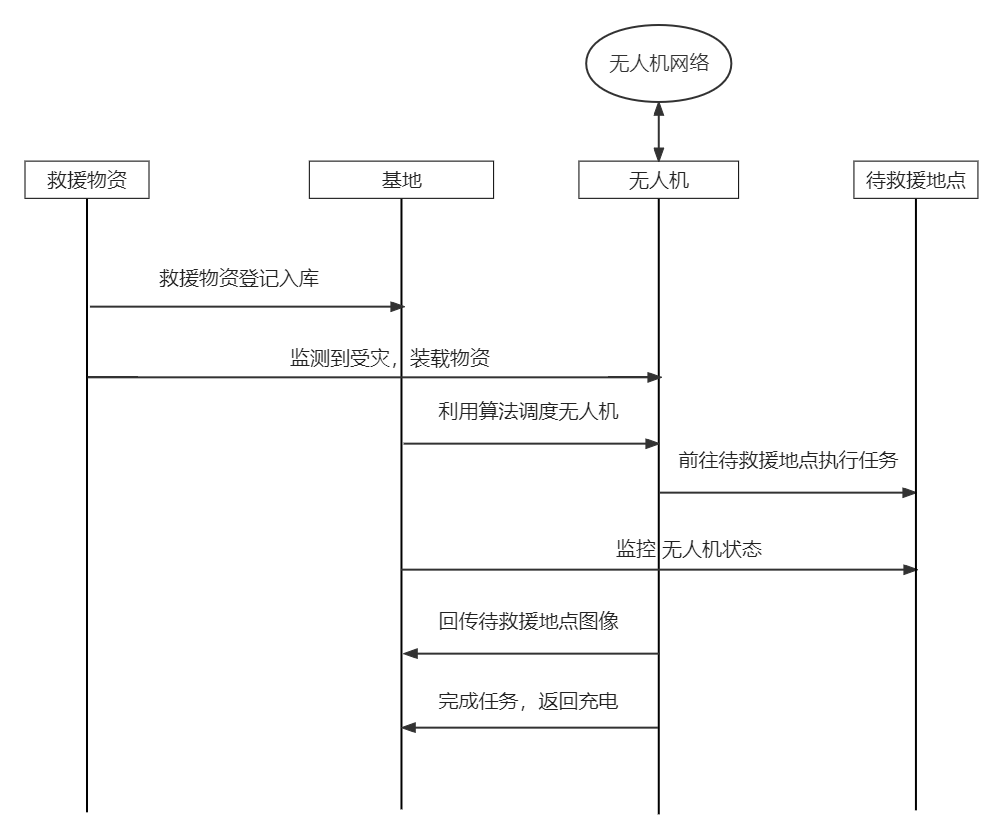
\includegraphics[width = 1.0\textwidth]{fg2_process}
	\caption{无人机紧急救援系统的主要工作流程}
	\label{fg202}
\end{figure}

\begin{itemize}
	\item [(1)]基地在收到新的一批救援物资后,会对救援物资的质量、体积和其他重要信息进行登记造册,存储在基地的物资管理系统中,
	以备查验和后续救援工作使用; 
	\item [(2)]基地的调度中心对无人机的型号、剩余续航时间和载重等信息进行检查,然后根据这些信息,使用算法计算出无人机的最佳调度方案。
	方案中包含无人机的路径规划、运输任务和飞行时间等关键信息;
	\item [(3)]由人工或者智能机器人对无人机进行物资装载,装载完成后,无人机从基地的起降中心出发,开始执行任务;
	\item [(4)]在任务执行过程中,无人机通过网络与基地进行通信,基地可以实时获取无人机的当前状态,同时无人机对拍摄的待救援地点状况进行回传;
	\item [(5)]无人机完成任务后,会与基地调度中心进行确认,待基地确认后,无人机进行返航,本次运送任务结束,待充电完成后准备进行下一次救援任务。
\end{itemize}

\section{问题模型的建立}[Establishment of Problem Model]

\subsection{基地}[Base]
在无人机紧急救援系统的问题模型中,基地使用$B$来表示。当上游救援物资到达基地时,$B$会记录救援物资的详细信息。
基地$B$作为无人机的调度中心和维护中心,会根据获取的信息指挥无人机将物资运送到各个待救援地点。
\subsection{待救援地点及其时间敏感性}[POI]
我们将待救援地点统称为兴趣点,在本问题中,无人机到兴趣点之间的距离与其时间敏感程度无明显关系,因此在设计算法时应该有效协调距离和时间敏感性之间的关系,
并据此对于无人机的路径规划进行决策。假设有$n$个兴趣点,用$P=\lbrace p_1, p_2, \cdots ,p_n \rbrace$进行表示。
这些兴趣点在目标区域内的分布是随机的,位置已知,且为静态。


由于不同的兴趣点其紧急情况不同,它们都有自身的时间敏感性$T_s=\lbrace ts_1, ts_2, \cdots ,ts_n \rbrace$。
我们考虑现实中的实际情况,这些兴趣点可能也会允许无人机在超时一定时间内到达,也将其视为成功救援,
所以我们设置一个公差系数$e$,认为无人机在$(1+e) \cdot t_si$时间内对兴趣点$p_i$进行了救援,即视为救援成功。
\subsection{救援物资}[Relief materials]
在无人机参与应急救援行动前,基地会采集各兴趣点的救援物资需求$S=\lbrace s_1, s_2, \cdots ,s_n \rbrace$, $s_i$代表兴趣点$p_i$所需要的的救援物资的质量。为了简化实验的
研究,我们忽视救援物资的体积,仅考虑救援物资的质量对无人机载重的影响。
\subsection{无人机}[UAV]
基地$B$中停放有$m$架型号相同的无人机,这些无人机用$U=\lbrace u_1, u_2, \cdots ,u_m \rbrace$进行表示,且它们拥有
相同的飞行速度$v$、最大载重$w$、单次飞行载重$w \prime$和最大续航时间$T_{max}$等基础参数。


为了研究的方便,本文在使用无人机执行紧急救援任务时,还对模型进行了适当简化:
\begin{itemize}
	\item [(1)] 无人机以固定速度$v$进行直线飞行,不考虑外界自然条件以及无人机状况对速度的影响;
 	\item [(2)] 不考虑救援物资的体积,只对无人机的载重进行考虑;
  	\item [(3)] 不考虑无人机在起飞和降落过程中对于电量的消耗和花费的时间,无人机从任务开始时即视为已经起飞并离开基地,无人机在完成任务后只要到达基地上方即视为已经返回基地并开始充电。
\end{itemize}

\section{评价指标}[Evaluating indicator]
前面提到,我们在判断无人机是否成功完成对兴趣点的救援时,引入了一个公差系数$e$,认为无人机在$(1+e) \cdot t_si$时间内对兴趣点$p_i$进行了救援,即视为救援成功。所以,我们在评价无人机对兴趣点的覆盖情况时,就有
两项指标:准时覆盖率$R_o$和有效覆盖率$R_e$。
\begin{equation}
R_o=\frac{\sum_{k=1}^m\sum_{i=1}^n o_{ik}}{n}
\end{equation}
\begin{equation}
R_e=\frac{\sum_{k=1}^m\sum_{i=1}^n e_{ik}}{n}
\end{equation}
其中,$o_{ik}$代表第$i$个兴趣点$p_i$是否被第$k$架无人机$u_k$准时覆盖。如果被准时覆盖,则$o_{ik} = 1$,反之$o_{ik} = 0$。
即准时覆盖率是被准时覆盖的兴趣点的数量与所有兴趣点的总数量$n$的比值。


而$e_{ik}$代表第$i$个兴趣点$p_i$是否被第$k$架无人机$u_k$有效覆盖。如果被有效时覆盖,则$e_{ik} = 1$,反之$e_{ik} = 0$。
即有效覆盖率是被有效覆盖的兴趣点的数量与所有兴趣点的总数量$n$的比值。

\section{对问题模型的概述}[Overview of problem model]
经过上面的分析,我们把问题模型定义为:给定一组兴趣点$P=\lbrace p_1, p_2, \cdots ,p_n \rbrace$。这些兴趣点随机地分布在目标区域内,他们拥有自己的时间敏感性$T_s=\lbrace ts_1, ts_2, \cdots ,ts_n \rbrace$
和对救援物资的需求量$S=\lbrace s_1, s_2, \cdots ,s_n \rbrace$。在无人机基地$B$中停放有$m$架无人机$U=\lbrace u_1, u_2, \cdots ,u_m \rbrace$,每架无人机拥有
相同的飞行速度$v$、最大载重$w$、单次飞行载重$w \prime$和最大续航时间$T_{max}$等基础参数。该问题的目标是最大化对兴趣点的准时覆盖率$R_o$和有效覆盖率$R_e$,同时以有效覆盖率$R_e$为最高优先级。
每架无人机在最大续航时间$T_{max}$内完成任务后,都会返回基地$B$,当所有可以被覆盖的兴趣点都完成覆盖后,即视为无人机应急救援任务完成。


对该问题的数学描述如下:

\begin{equation}
 {max}\quad{R_e} 
\end{equation}


从属于:


\begin{equation}
	T_k(i) \le (1+e) \cdot ts_i
\end{equation}
\begin{equation}
	{\forall} k\in \lbrace u_1, u_2, \cdots ,u_m \rbrace ,{\forall} i \in \lbrace p_1, p_2, \cdots ,p_n \rbrace,0\le e \le1
\end{equation}
\begin{equation}
	T_k = \sum_{i=1}^n x_{ik}t_i \le T_{max}
\end{equation}
\begin{equation}
	{\forall} k\in \lbrace u_1, u_2, \cdots ,u_m \rbrace
\end{equation}
\begin{equation}
	w \prime \le w
\end{equation}

\section{本章小结}[Brief summary] 
本章主要建立了无人机紧急救援系统的模型,提出了一套无人机救援任务调度方案,并对整个系统的设计方案和工作流程进行了介绍。
接下来,依次对该系统中的模型进行了介绍,并使用数学符号表示了相关元素,并用数学方式表示了问题中的目标函数和约束等。



% 第3章
% !TEX root = ../main.tex

% 中英标题:\chapter{中文标题}[英文标题]
\chapter{带载重的贪婪成本选择算法设计与实现}[Model Solving Scheme Based on Improved Greedy Algorithm]

\section{贪婪式成本选择算法的改进}[Improved algorithms]
相比设计时参考的贪婪成本选择(Greedy Cost Selection, GCS)算法,本算法主要有以下方面的改进:
% \begin{itemize}
%	\item [(1)] 代价函数重新调整了权重,无人机续航时间与兴趣点存活时间之间的关系对于无人机访问兴趣点的先后顺序的影响权重较大,所以提高了该项数据在代价函数中的优先级,
%	同时代价函数中加入了载重相关的因素,尽量防止无人机的路径规划中存在有无人机超重运输的情况;
%	\item [(2)] 优化了路径规划的顺序,同时考虑m架无人机访问兴趣点的代价,再进行线路的规划,可以提高无人机对于兴趣点的有效覆盖率和准时率;
%	\item [(3)] 在无人机返回基地之前,若还有空余续航时间,仍然会访问已超时的兴趣点,从而实现对兴趣点的全覆盖。
% \end{itemize}
\begin{itemize}
	\item [(1)] 对于代价函数进行了权重的重新设计。在原本的问题设计中,没有考虑无人机的载重上限$w$对无人机路径规划的影响。由于无人机载重有限,所以对物资需求量越高的兴趣点,无人机访问该兴趣点的成本也就更高。在代价函数重新设计后,影响代价函数的主要因素有
无人机飞行前往兴趣点所需要的时间、兴趣点的时间敏感性和兴趣点对物资的需求量。由于问题中最需要保证的就是无人机对兴趣点的有效覆盖率$R_e$,因此将兴趣点的时间敏感性放在首要优先级,兴趣点对物资的需求量放在次要优先级,而无人机飞行前往兴趣点所需要的时间也进行适当考虑。
故系数的选择为$\alpha = 10,\beta = 100,\gamma = 50$;
	\item [(2)] 无人机在完成任务后,若还有剩余的续航时间,会尝试访问已经超时的兴趣点,从而实现了对于兴趣点的完全覆盖;
\end{itemize}


由于相较GCS算法,改进后的算法主要增加了对无人机载重情况的考虑,故本文将其命名为带载重的贪婪成本选择算法(Greedy Cost Selection Algorithm With Load, GCSAWL)。

\section{带载重的贪婪成本选择算法的描述}[Algorithm th]
带载重的贪婪成本选择算法属于贪婪式算法,使用GCSAWL对模型进行求解的基本思想是,在一次救援任务中依次为每架无人机生成扫描覆盖路径,每条扫描覆盖路径的起点和终点均为基地$B$。在路径规划过程中,本文设计了一个成本函数来计算访问每个兴趣点的成本。
该成本函数考虑了访问兴趣点所需的时间、该兴趣点的时间敏感性$T_s$、当前无人机的扫描覆盖进度和载重等因素。在路径规划时,本文采用贪婪策略,每次都选择覆盖成本最低的兴趣点,从而为当前无人机获得最佳的扫描路径。


在无人机出发之前,首先需要检查兴趣点的时间敏感性$T_s$是否合理。如果兴趣点$i$的时间敏感性$ts_i$比无人机从基地$B$至该兴趣点的直线飞行时间$\frac{d_{iB}}{v}$小,则说明无论如何无人机都无法在准确时间内对该兴趣点进行访问,
需要重新检查时间敏感性。接下来,逐个对$m$架无人机规划扫描路径$O=\lbrace o_1, o_2, \cdots ,o_m \rbrace$进行规划。第$k$架无人机的初始扫描路径$O_k$为$\emptyset$。变量$T_k$用于记录无人机在起飞后所花费的时间,其初始值
为无人机在上升阶段所花费的时间$T_a$。对于$P$中的每个兴趣点$p_i$,本文首先判断这个兴趣点是否满足兴趣点可访问的三个条件。第一个条件是当无人机飞到兴趣点$p_i$时,该兴趣点仍然存活,也就是说时间在可接受范围$(1+e) \cdot ts_i$内。
第二个条件是,当无人机执行完任务后,剩余的续航里程可以让无人机返回至基地$B$进行充电和维护等作业。第三个条件是无人机在执行任务时不能超重运输。只有当这三个条件同时满足时,本文才说兴趣点$p_i$是可访问的。


然后,本文设计了一个成本函数来评估无人机访问$p_i$的成本:
\begin{equation}
	\varphi = \frac{T_k}{T_{max}}
\end{equation}
\begin{equation}
	C_i = \alpha t_i + \beta (ts_i - T_k)^\varphi + \gamma s_i
\end{equation}

系数$\varphi$反映当前无人机的扫描覆盖任务完成进度。$(ts_i - T_k)$表示兴趣点$p_i$的剩余访问时间,扫描覆盖任务越接近结束,访问兴趣点的优先级越高,剩余的访问时间越短。$s_i$代表的是兴趣点$p_i$所需求的救援物资质量。
$\alpha,\beta,\gamma$是系数,负责调节三个影响因素的权重。在成本函数中,距离当前位置近、剩余可访问时间短且载重要求低的兴趣点访问成本最低,将首先被访问。如果该兴趣点不可访问,则会将$C_i$设置为$+\infty$。计算完所有兴趣点
的成本后,选择访问成本最小的兴趣点$p_j$,然后将$p_j$添加到路径$O_k$中,并将其从$P$中删除,更新计时器$T_k$,并判断兴趣点$p_j$的准时覆盖情况和有效覆盖情况。


如果$p_j$不存在,即当前$P$中所有的兴趣点成本均为$+\infty$,则意味着没有兴趣点可以被继续覆盖,在这种情况下,本文还可以要求无人机在不超重且续航里程足够的情况下,访问较近的已超时但未被访问的兴趣点,实现对所有兴趣点的尽可能的覆盖。
完成任务后,无人机$u_k$应返回基地$B$,当$u_k$返回基地或已经没有剩余的未被访问的兴趣点时,$u_k$的路径规划完成。


最后,在全部$m$架无人机的路径都被规划完成后,根据第二章中提到的公式计算有效覆盖率$R_e$和准时覆盖率$R_o$,算法结束。


算法的伪代码如下:
 
\begin{algorithm}[H]  %其中这里面不能有H不然会报错,不过不影响结果
	\caption{带载重的贪婪成本选择算法}%算法名字
	\LinesNumbered %要求显示行号
	\KwIn{兴趣点的集合$P$,兴趣点对应时间敏感性的集合$T_s$,兴趣点对应的救援物质需求的集合$S$,无人机的集合$U$,基地$B$,无人机的最大续航时间$T_{max}$,无人机的飞行速度$v$,最大载重$w$。}%输入参数
	\KwOut{无人机的飞行路径规划$O$,无人机的准时覆盖率$R_o$和有效覆盖率$R_e$}%输出
	检查$T_s$的值是否符合要求\; %\;用于换行
	\For{$k=1 \rightarrow m$}{
		设置$O_k = \emptyset$、$T_k = 0$和无人机是否完成覆盖的标识符\;
		\While{$P \ne \emptyset ~ and ~ B_0\notin ~  O_k $}{
		\For{$p_i \in P$}{
			计算无人机的直线飞行至下一个兴趣点的飞行时间$t_i$\;
			\eIf{$\enspace T_k + t_i \le (1+e)\cdot ts_i \enspace and \enspace T_{max} - T_k \ge 0 \enspace and \enspace w \prime \le w \enspace$}{
			$\varphi =  T_k / T_{max}$\;
			$C_i = \alpha t_i + \beta (ts_i - T_k)^\varphi + \gamma m_i$\;
		}{
			$C_i = +\infty$\;
		}
		}
		选择C最小的$p_j \in P$\;
		\eIf{$p_j$存在}{
			将$p_j$添加至$O_k$,将$p_j$从$P$中移除\;
			$T_k = T_k + t_j$\;
			判断兴趣点覆盖情况,设置相关标识符\;
		}{
			将$B$添加至$O_k$\;
		}
		
	}
	}
	计算无人机的准时覆盖率$R_o$和有效覆盖率$R_e$\;
	return $O,R_o,R_e$
\end{algorithm}


\section{带载重的贪婪成本选择算法的复杂度分析}[Complexity Analysis of Algorithm]
在带载重的贪婪成本选择算法中,计算$P$中所有兴趣点的访问成本的部分其时间复杂度为$O(n)$,因为$P$有$n$个兴趣点。同样,将兴趣点添加到无人机的扫描路径的过程,其时间复杂度也为$O(n)$。最后,在规划$m$架无人就的扫描路径时,迭代次数为$m$,故
本算法的时间复杂度为$O(mn^2)$。


\section{本章小结}[Brief summary]
在本章中,主要介绍了使用带载重的贪婪成本选择算法解决带时间窗的无人机扫描覆盖问题的基本思想和算法细节。该算法针对贪婪成本选择算法进行了改进,以更符合实际情况和提高算法性能,同时对该算法的复杂性进行了分析。

% 第4章
% !TEX root = ../main.tex

% 中英标题:\chapter{中文标题}[英文标题]
\chapter{基于改进的遗传算法的模型求解方案}[Model Solving Scheme Based on Improved Genetic Algorithm]

\section{算法设计}[Algorithm design]

\subsection{染色体的编码方法}[Method of chromosome coding]
在遗传算法中,染色体的编码方法主要有二进制编码法、符号编码法和自然数编码法等。在本问题中,我们选择的是自然数编码法。


自然数编码由自然数$1,2,\cdots,n$组成,这些基因位代表的是兴趣点,而基因的序列则代表无人机对兴趣点的访问顺序。$0$在编码中表示的是基地$B$,由于无人机从基地$B$出发,
完成配送任务后又返回基地$B$,因此单架无人机的访问顺序总是从$0$开始,而又从$0$结束。基地$B$的编码$0$又可以很方便地将不同无人机的线路分离。自然数编码能够很好地反映
无人机参与救援的过程,便于后面代码的撰写,因此选择了该编码方法。


在本问题中,基地$B$中停放有$m$架无人机,对$n$个兴趣点实施救援。由于在整个流程中,每个兴趣点只被访问一次,所以无人机的数量决定了子路径的数量,从而本问题中一条染色体的长度
为$k+n+1$。例如,一条染色体的编码为``0 7 8 0 4 5 6 0 1 3 2 0 9 0'',这代表$4$架无人机同时对$9$个兴趣点进行救援,所有的子路径为:
$$0\rightarrow7\rightarrow8\rightarrow0,0\rightarrow4\rightarrow5\rightarrow6\rightarrow0,0\rightarrow1\rightarrow3\rightarrow2\rightarrow0,0\rightarrow9\rightarrow0$$

\subsection{种群的初始化设计}[Population initialization design]
初始化种群时,我们采用随机访问的方法进行设计。首先随机产生一条无人机的配送子路径,如果无人机根据这条路径运送救援物资能够不超出无人机的最大载重$w$,则存储这条路径,反之抛弃这条路径,
然后重复这个过程,直到所有的兴趣点都被无人机访问。


将以上的子路径组合起来,并将基地$B$用自然数$0$进行表示,连接这些子路径,可以得到一条包含所有兴趣点的染色体,这个染色体就是一套完整的无人机调度方案。在本问题中,我们将初始种群个数设置为
$100$,即在初始化过程中会产生$100$条符合要求的染色体。

\subsection{适应度函数设计}[Design of fitness function]
使用自然数对染色体进行编码,可以保证无人机的飞行路径较为清晰,但是不能确保在进化过程中产生的新路径能够一定满足不超重和尽可能少超时,所以为了确保进化过程中能产生最优解,我们需要引入一个惩罚函数,
对不合理的路径规划结果进行惩罚:
$$ f= \alpha d_s + \beta m_s + \gamma w_s $$


其中,$d_s$是无人机的飞行距离之和,$m_s$是所有子路径中无人机的超重数量之和,$w_s$是所有子路径中无人机超出时间窗之和。而$\alpha,\beta,\gamma$是系数,根据各参数的重要性,将这些参数设置为
$\alpha = 1,\beta = 10,\gamma = 100$。


由于各参数的单位不统一,在计算惩罚函数时还需要对数据进行归一处理。


所有子路径中无人机超出时间窗之和$w_s$用以下公式表示:
$$ w_s = \sum_{i=1}^n max\left\{\Delta t_i,0\right\}$$


其中,$\Delta t_i$代表无人机从起飞到访问兴趣点$p_i$所花费的时间与该兴趣点的时间窗$ts_i$之差。


为了衡量个体的适应度,将适应度函数$F$设置为惩罚函数$f$的倒数:
$$ F = \frac{1}{f}$$

\subsection{对个体的择优}[Individual preference]
为了更好地模拟孟德尔豌豆实验,在算法中加入了对优秀个体自花授粉的过程。将初始化种群中的100个个体按照适应度大小进行排序,选择其前
$5\%$的的染色体进行自交,而其余的染色体则进入选择阶段。在自交过程中,会产生2倍数量的个体,他们跳过选择阶段,直接进入变异过程,这样可以有效
保护优秀基因。

\subsection{选择过程}[selection process]
采用轮盘赌算法进行个体的选择。轮盘赌算法是一种回放式的随机采样方法,个体进入下一代的概率就是其适应度与整个种群个体适应度之和的比值,适应度的值越大,个体被选中的概率也就越大。
但是,传统轮盘赌算法误差较大,部分个体容易被多次选出,可能会削弱种群的规模和降低种群多样性,导致最终陷入局部最优解。为了避免这种情况,本文对轮盘赌算法进行了一些改进:
$$ F_i' = F_i - F_{min} $$


其中,$F_i$是第$i$个个体的适应度,$F_{min}$是所有个体中适应度的最小值,其计算方法如下:
$$ F_{min} = min\left\{F\right\} $$


最后,可以计算出第$i$条染色体被选择的概率为:
$$ P(i) = \frac{F_i}{\sum F_i'} $$

\subsection{交叉操作}[Crossover operation]
在遗传算法中,交叉操作是指满足交叉概率$p_c$两个相互配对的染色体交换部分基因,形成新的个体。常用的交叉方式有单点交叉、两点交叉、多点交叉和均匀交叉等。由于该问题的特殊性,所有存在无人机超重情况的规划路径都
应该被剔除,因此这里在进行交叉操作时,需要使得结果尽量避免存在有无人机在运输过程中超重,交叉过程如\figref{fg401}所示:
\begin{figure}[ht]
	\centering
	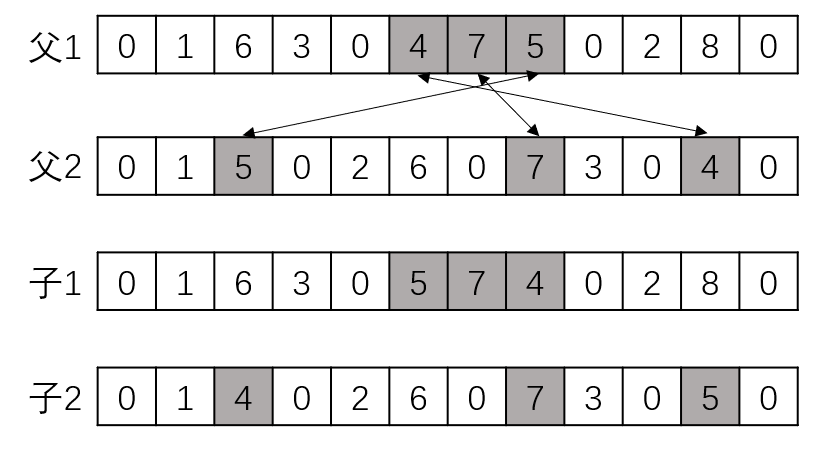
\includegraphics[width = 0.7\textwidth]{fg3_jiaocha}
	\caption{交叉操作过程示例}
	\label{fg401}
\end{figure}


\begin{itemize}
	\item [(1)] 针对满足交叉概率$p_c$的父代个体1和父代个体2,从父代个体1中随机选择一个子路径作为交叉片段(不包括子路径中的自然数0);
	\item [(2)] 从父代个体2中寻找与上述子路径编号对应的片段,作为父代个体2的交叉片段;
	\item [(3)] 交换父代个体1和父代个体2的交叉片段,得到子代个体1和子代个体2;
 	\item [(4)] 重复上述步骤,直到生成子代的数量符合要求。
\end{itemize}

\subsection{变异操作}[Mutation operation]
针对满足变异概率$p_m$的染色体,在兴趣点编号范围内随机选出两个不相同且不为0的数字,将染色体对应的基因编码进行交换,即为变异过程。变异过程如\figref{fg402}所示。
\begin{figure}[ht]
	\centering
	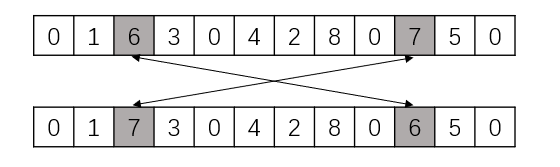
\includegraphics[width = 0.7\textwidth]{fg4_bianyi}
	\caption{变异操作过程示例}
	\label{fg402}
\end{figure}
\subsection{对基因的多轮筛选}[Multiple rounds of gene screening]
在种群初始化、交叉算子和变异算子后,选择对各条路径的载重约束进行检查。如果发现有个体对应的路径存在无人机超重配送的情况,应该对染色体予以删除,以符合无人机的飞行安全要求。

\section{算法的伪代码}[Pseudocode of the algorithm]
\begin{algorithm}[H]
\caption{改进的遗传算法}
\LinesNumbered %要求显示行号
\KwIn{\rm video \ \it X,\ \rm hole \ \it H,\ \rm validity \ \it V \\}
\KwOut{\rm complection \ video \it Y \\ }
\For{condition}{
	only if\;
	\If{condition}{
		1\;
	}
}
\end{algorithm}

\section{算法的复杂度分析}[Complexity Analysis of Algorithm]

\section{算法的改进}[Improved algorithms]
与传统的遗传算法相比,本文提出的算法有以下改进点:
\begin{itemize}
	\item [(1)] 在算法中加入多轮筛选,对不符合无人机载重要求的个体予以删除,符合优质个体多繁衍,劣质个体少繁衍甚至不繁衍的自然选择规律;
	\item [(2)] 类似孟德尔豌豆杂交实验,在适应度计算完成后对优秀的个体进行自花授粉,以保留优秀个体的基因;
	\item [(3)] 对轮盘赌选择方法进行了改进,避免削弱种群的规模和降低种群多样性,防止陷入局部最优解;
 	\item [(4)] 对交叉过程进行了改进,尽量避免了交叉过程后存在有无人机在运输过程中超重的问题。
\end{itemize}
\section{本章小结}[Brief summary]
本章主要对遗传算法的基本流程进行了介绍,并且针对传统遗传算法不足之处进行了一些改进,提出了一种改进的遗传算法以解决带时间敏感的无人机扫描覆盖问题,该算法便于找到更优秀的最终解。

% 第5章
% !TEX root = ../main.tex

\chapter{仿真实验及结果分析}[Simulation Experiment and Result Analysis]

\section{仿真实验的参数设置}[Parameter setting]

本次实验的仿真于个人PC上完成,操作系统为Microsoft Windows 11 x64 专业版 21H2,内存大小为16.00GB,CPU型号为AMD Ryzen 7 5800H,使用编程语言版本为Python 3.9.12,IDE版本为PyCharm 2021.3.1。


在实验的模拟中,模拟的目标区域是边长为50km的正方形,无人机基地$B$位于该区域的中心。在该区域内兴趣点随机分布,每个兴趣点的需求物资量也随机产生。无人机的最大续航时间为180分钟,最大载重为100kg,
其中从基地起飞和降落的时间忽略不计。每架无人机的移动速度$v$设置为25m/s。为了更好地得知算法的性能,本文设置了实验组(一):
\begin{itemize}
	\item [(1)] 比较在无人机数量$m$改变,兴趣点数量$n$不变,兴趣点的时间敏感性$T_s$随机范围固定,兴趣点的物资需求$S$随机范围固定的条件下,带载重的贪婪成本选择算法、经典遗传算法和带自交的遗传算法共三种算法的有效覆盖率;
    \item [(2)] 比较在兴趣点数量$n$改变,无人机数量$m$不变,兴趣点的时间敏感性$T_s$随机范围固定,兴趣点的物资需求$S$随机范围固定的条件下,带载重的贪婪成本选择算法、经典遗传算法和带自交的遗传算法共三种算法的有效覆盖率;
    \item [(3)] 比较在兴趣点的时间敏感性$T_s$随机范围改变,兴趣点数量$n$不变,无人机数量$m$不变,兴趣点的物资需求$S$随机范围固定的条件下,带载重的贪婪成本选择算法、经典遗传算法和带自交的遗传算法共三种算法的有效覆盖率;
\end{itemize}


为了更好地比较三种算法间的性能差异,还设置了实验组(二):
\begin{itemize}
	\item [(1)] 在其他参数不变的情况下,比较带载重的贪婪成本选择算法和改进前后遗传算法结果的无人机总飞行里程;
    \item [(2)] 在其他参数不变的情况下,比较带载重的贪婪成本选择算法和改进前后遗传算法结果的无人机总飞行时间。
\end{itemize}


为了更好地比较经典遗传算法和带自交的遗传算法间的性能差异,还设置了实验组(三):
\begin{itemize}
	\item [(1)] 在其他参数不变的情况下,逐次增加遗传算法的迭代次数,比较改进前后遗传算法的准时覆盖率和有效覆盖率;
 	\item [(2)] 在其他参数不变的情况下,逐次增加遗传算法的迭代次数,比较改进前后遗传算法结果中违反载重约束的路径数量变化。
\end{itemize}
\section{GCSAWL算法与GAWS算法的性能对比与实验结果分析}[Algorithm Comparison]
实验组(一):待救援区域为边长50km的正方形,基地$B$位于$(0,0)$,无人机的飞行速度为25m/s,最大载重为100kg,遗传算法的迭代次数为50次。
\begin{itemize}
    \item [(1)] 兴趣点的数量$n$设置为100,兴趣点的时间敏感性$T_s$随机范围为(60mins,150mins),物资需求$S$随机范围为(5kg,15kg),无人机的数量$m$设置为0至10,实验结果如\figref{fg501}所示:
    \begin{figure}[H]
        \begin{center}
            \begin{tikzpicture}
                \begin{axis}
                    %坐标系配置,只显示左边坐标轴
                    [axis lines = left, xlabel = {无人机数量(架)}, ylabel = {有效覆盖率},tick align=outside,legend style={at={(1.5,0.75)},anchor=north}]
                    %绘制曲线-2
                    \addplot+[smooth,green,mark=square]
                    coordinates{
                        (0,0) (1,0.1600) (2,0.2200)
                        (3,0.3000) (4,0.3700)(5,0.4700)
                        (6,0.5600) (7,0.6500)(8,0.7500)
                        (9,0.84) (10,0.9200)
                    };
                    \addlegendentry{带载重的贪婪成本选择算法}; %绘制标注
                    %绘制曲线-3
                    \addplot+[smooth,blue,mark=x]
                    coordinates{
                        (0,0) (1,0.1050) (2,0.1800)
                        (3,0.2932) (4,0.3945)(5,0.4987)
                        (6,0.6021) (7,0.7105)(8,0.7834)
                        (9,0.87) (10,0.96)
                    };
                    \addlegendentry{经典遗传算法}; %绘制标注
                    %绘制曲线-4
                    \addplot+[smooth,cyan,mark=+]
                    coordinates{
                        (0,0) (1,0.1100) (2,0.1900)
                        (3,0.3128) (4,0.4373)(5,0.5191)
                        (6,0.6323) (7,0.7491)(8,0.8252)
                        (9,0.9200) (10,1)
                    };
                    \addlegendentry{带自交的遗传算法}; %绘制标注
                \end{axis}
            \end{tikzpicture}
        \end{center}
        \caption{三种算法的覆盖率随无人机数量的变化情况}
        \label{fg501}
    \end{figure}
    实验结果说明,在无人机数量较低时,带载重的贪婪成本选择算法的有效覆盖率$R_e$结果比其余两种遗传算法要高,但当无人机数量增加后,带自交的遗传算法的有效覆盖率$R_e$平均较带载重的贪婪成本选择算法提高约7\%至9\%,较经典遗传算法平均提高约5\%。
    \item [(2)]无人机的数量$m$设置为10,兴趣点的时间敏感性$T_s$随机范围为(60mins,150mins),
    物资需求$S$随机范围为(5kg,15kg),兴趣点的数量$n$设置为25、50、75、100、150、200、250、300、350、400、450和500,实验结果如\figref{fg502}所示:
    \begin{figure}[H]
        \begin{center}
            \begin{tikzpicture}
                \begin{axis}
                    %坐标系配置,只显示左边坐标轴
                    [xlabel = {兴趣点数量(个)}, ylabel = {有效覆盖率},tick align=outside,legend style={at={(1.5,0.75)},anchor=north},ytick={0,0.1,0.2,0.3,0.4,0.5,0.6,0.7,0.8,0.9,1}]
                    %绘制曲线-2
                    \addplot+[smooth,green,mark=square]
                    coordinates{
                        (0,1) (25,1) (50,1)
                        (75,1) (100,0.9500)(150,0.6400)
                        (200,0.495) (250,0.408)(300,0.34)
                        (350,0.3029) (400,0.2450)(450,0.2267)(500,0.1960)
                    };
                    \addlegendentry{带载重的贪婪成本选择算法}; %绘制标注
                    %绘制曲线-3
                    \addplot+[smooth,blue,mark=x]
                    coordinates{
                        (0,1) (25,1) (50,1)
                        (75,1) (100,0.9800)(150,0.6867)
                        (200,0.5050) (250,0.430)(300,0.3633)
                        (350,0.3000) (400,0.2500)(450,0.2500)(500,0.2200)
                    };
                    \addlegendentry{经典遗传算法}; %绘制标注
                    %绘制曲线-4
                    \addplot+[smooth,cyan,mark=+]
                    coordinates{
                        (0,1) (25,1) (50,1)
                        (75,1) (100,1)(150,0.7178)
                        (200,0.5508) (250,0.4609)(300,0.3726)
                        (350,0.3258) (400,0.2784)(450,0.2763)(500,0.2406)
                    };
                    \addlegendentry{带自交的遗传算法}; %绘制标注
                \end{axis}
            \end{tikzpicture}
        \end{center}
        \caption{三种算法的覆盖率随兴趣点数量的变化情况}
        \label{fg502}
    \end{figure}
    从实验结果可以看出,随着兴趣点数量的增加,少量的无人机难以对大量的兴趣点实现有效覆盖,因此有效覆盖率$R_e$的整体趋势是下降的。但是,尽管三种算法的有效覆盖率$R_e$
    都在不断下降,带自交遗传算法的有效覆盖率$R_e$始终高于其余两种算法,体现出其性能的优越性。
    \item [(3)]无人机的数量$m$设置为5,兴趣点的数量$n$设置为100,兴趣点的时间敏感性$T_s$随机范围为(20mins,120mins),(60mins,150mins)和(90mins,180mins)三组,物资需求$S$随机范围为(5kg,15kg),实验结果如表\ref{table2}所示:
    \begin{table}[htbp]
        \vspace{0.5em}\centering\wuhao
        \caption{三种算法的有效覆盖率对比}\label{table2}
        \begin{tabular}{cccc}
        \toprule[1.5pt]
        算法名称 & (20mins,120mins) & (60mins,150mins) & (90mins,180mins) \\
        \midrule[1.5pt]
        带载重的贪婪成本算法 & 54.21\% & 62.18\% & 69.54\%\\
        经典遗传算法 & 56.78\% & 63.47\% & 71.98\% \\
        带自交的遗传算法 & 59.23\% & 67.32\% & 73.45\% \\
        \bottomrule[1.5pt]
        \end{tabular}
        \end{table}
    
    
        实验结果说明了有效覆盖率$R_e$与时间敏感性范围$T_s$之间的关系。时间敏感性范围(20mins,120mins)说明有一些兴趣点的最低时间可能只有20分钟,这意味着无人机很难去覆盖这些兴趣点。
    而从结果来看,带自交的遗传算法在(20mins,120mins)、(60mins,150mins)和(90mins,180mins)三个区间内有效覆盖率$R_e$均比带载重的贪婪成本算法和经典遗传算法高。
\end{itemize}


实验组(二):待救援区域为边长50km的正方形,基地$B$位于$(0,0)$,无人机的数量为5架,兴趣点的数量为50,无人机的飞行速度为25m/s,最大载重为100kg,兴趣点的时间敏感性随机范围为(50mins,140mins),物资需求随机范围为(5kg,15kg)。遗传算法的迭代次数为50次。


实验结果如表\ref{table3}所示:
\begin{table}[htbp]
    \vspace{0.5em}\centering\wuhao
    \caption{三种算法的无人机总飞行里程和时间对比}\label{table3}
    \begin{tabular}{ccc}
    \toprule[1.5pt]
    算法名称 & 总飞行时间(mins) & 总飞行里程(km) \\
    \midrule[1.5pt]
    带载重的贪婪成本选择算法 & 266.88 & 400.33 \\
    经典遗传算法 & 243.05 & 364.58 \\
    带自交的遗传算法 & 234.63 & 351.95 \\
    \bottomrule[1.5pt]
    \end{tabular}
    \end{table}


实验结果表明,三种算法除准时覆盖率$R_o$和有效覆盖率$R_e$的结果有明显差异外,改进后的遗传算法总飞行时间和总飞行里程下降了约3.6\%,且两种遗传算法的总飞行时间和总飞行里程均低于带载重的贪婪成本选择算法,
这符合课题中优先提高准时覆盖率$R_o$和有效覆盖率$R_e$的同时也要考虑降低无人机总飞行时间和总飞行里程,以降低无人机救援成本的目标。

实验组(三):待救援区域为边长50km的正方形,基地$B$位于(0,0),无人机的数量为8架,兴趣点的数量为100,无人机的飞行速度为25m/s,最大载重为100kg,兴趣点的时间敏感性随机范围为(80mins,150mins),物资需求随机范围为(5kg,15kg)。遗传算法的迭代次数从0增加到50。
\begin{itemize}
    \item [(1)]可以看到,如\figref{fg503}所示,在迭代次数小于20次时,此时改进前后遗传算法的准时覆盖率$R_o$和有效覆盖率$R_e$没有明显的差异,
    而当迭代次数逐次增加,改进的遗传算法拥有更好的覆盖率,且改进后的遗传算法在40次迭代后已经得到最优解,而改进前的遗传算法需要进行50次迭代后才能得到最优解。
    \begin{figure}[H]
    \begin{center}
        \begin{tikzpicture}
            \begin{axis}
                %坐标系配置,只显示左边坐标轴
                [axis lines = left, xlabel = {迭代次数}, ylabel = {覆盖率},tick align=outside,legend style={at={(1.5,0.75)},anchor=north}]
                %绘制曲线-1
                \addplot+[smooth,red,mark=triangle]
                coordinates{
                    (0,0.1425) (10,0.2242) (20,0.5245)
                    (30,0.6741) (40,0.7545)(50,0.7912)
                };
                \addlegendentry{经典遗传算法$\enspace R_o$}; %绘制标注
                %绘制曲线-2
                \addplot+[smooth,orange,mark=triangle]
                coordinates{
                    (0,0.1523) (10,0.2612) (20,0.5924)
                    (30,0.7541) (40,0.8645)(50,0.8702)
                };
                \addlegendentry{带自交的遗传算法$\enspace R_o$}; %绘制标注
                %绘制曲线-3
                \addplot+[smooth,blue,mark=*]
                coordinates{
                    (0,0.1425) (10,0.3442) (20,0.6545)
                    (30,0.8041) (40,0.9345)(50,1)
                };
                \addlegendentry{经典遗传算法$\enspace R_e$}; %绘制标注
                %绘制曲线-4
                \addplot+[smooth,purple,mark=*]
                coordinates{
                    (0,0.1537) (10,0.3612) (20,0.6924)
                    (30,0.8541) (40,1)(50,1)
                };
                \addlegendentry{带自交的遗传算法$\enspace R_e$}; %绘制标注
            \end{axis}
        \end{tikzpicture}
    \end{center}
    \caption{三种算法的覆盖率随迭代次数的变化情况}
    \label{fg503}
\end{figure}
    \item [(2)]在该组实验参数下,由于有8架无人机参与救援物资运输,故一共会产生8条无人机的配送路径,这里需要统计在迭代过程中这8条路径违反载重约束的情况。实验结果如\figref{fg504}所示。
\begin{figure}[H]
    \begin{center}
        \begin{tikzpicture}
            \begin{axis}
                %坐标系配置,只显示左边坐标轴
                [axis lines = left, xlabel = {迭代次数}, ylabel = {违反载重约束线路数量},tick align=outside,legend style={at={(1.5,0.75)},anchor=north}]
                %绘制曲线-1
                \addplot+[smooth,red,mark=triangle]
                coordinates{
                    (0,7) (5,5) (10,6)
                    (15,4) (20,3)(25,4)
                    (30,2) (35,1)(40,1)
                    (45,0) (50,0)
                };
                \addlegendentry{经典遗传算法$\enspace$违约线路数量}; %绘制标注
                %绘制曲线-2
                \addplot+[smooth,orange,mark=triangle]
                coordinates{
                    (0,7) (5,5) (10,4)
                    (15,1) (20,2)(25,1)
                    (30,0) (35,0)(40,0)
                    (45,0) (50,0)
                };
                \addlegendentry{带自交的遗传算法$\enspace$违约线路数量}; %绘制标注
            \end{axis}
        \end{tikzpicture}
    \end{center}
    \caption{改进前后遗传算法违约路径数量随迭代次数的变化情况}
    \label{fg504}
\end{figure}
\qquad 从实验结果可以得出结论,由于改进的遗传算法在进化过程中加入了符合“优胜劣汰”原则的多轮筛选过程,
使得违反载重约束的个体不易进入下一代参与进化,故改进后的遗传算法能在较少的迭代次数内将违反载重约束的降至0。
\end{itemize}
\section{本章小结}[Brief summary]
本章主要对带时间敏感性的无人机网络扫描覆盖问题进行了实验测试。根据对现实生活中实际情况的调查和研究,
设置了实验参数,并用带载重的贪婪成本选择算法、经典遗传算法和带自交的遗传算法进行了求解。
通过对实验结果的分析,本文发现两种遗传算法的有效覆盖率$R_e$均比带载重的贪婪成本选择算法高,且无人机飞行成本(以飞行里程和时间计)均比带载重的贪婪成本选择算法低。
同时,改进后的带自交的遗传算法的有效覆盖率$R_e$比改进前高,无人机飞行成本比改进前低。



% 第6章
% !TEX root = ../main.tex

% 中英标题:\chapter{中文标题}[英文标题]
\chapter{无人机紧急救援模拟系统}[UAV emergency rescue simulation system]

\section{需求分析}[demand analysis]

\subsection{任务目标}[en title]
无人机紧急救援模拟系统是整个无人机救援调度系统的重要组成部分,可以将其视为系统的前端部分。该系统
可以帮助基地中的管理人员更好地了解无人机的实际调度情况和任务分配情况,模拟无人机的物资投放过程。
\subsection{需求详解}[en title]
本系统主要需要实现的功能有待救援地点参数的设置、无人机参数的设置、区域地图显示、前后端功能交互等。
\begin{itemize}
	\item [(1)] 待救援地点参数的设置


    \qquad 用户可以在页面中手动添加待救援点的编号、时间敏感性、位置和名称等信息,也可以通过csv文件批量导入地点信息;
    \item [(2)] 无人机参数的设置
    

    \qquad 无人机的参数主要指的是在该区域内同时工作的无人机的数量、无人机的型号、载重和续航里程等信息;
    \item [(3)] 区域地图显示
    

    \qquad 用户选择待救援区域的大致范围后,页面将会显示该区域的实际地图,同时无人机、待救援点等地图要素同样会在地图上显示;

    \item [(4)] 前后端功能交互
    

    \qquad 在用户手动输入或批量导入参数信息后,通过页面中的“提交”按钮,前端将地图信息和各种参数传输至后端服务器,由服务器计算
    最优的无人机扫描覆盖路径,再将其传输至前端以供展示最终结果。
\end{itemize}
\section{设计概要}[design brief]
\subsection{系统框架}[en title]
该系统基于Web设计,使用B/S设计模式,其特点是客户端与服务端分离,通过通信协议进行数据传输,两者内部的实现是独立的,能够降低开发难度和维护难度。前端界面运行于用户浏览器中,使用HTML、CSS和JavaScript实现,并使用Ajax向后端发送和接收数据信息。后端使用Flask框架设计,负责路径规划的计算以及其他后台服务。
本系统中用户只需要选择区域,设置好相关参数,即可开始使用所有的功能。


本系统的设计框架如\figref{fg601}所示:

\begin{figure}[ht]
	\centering
	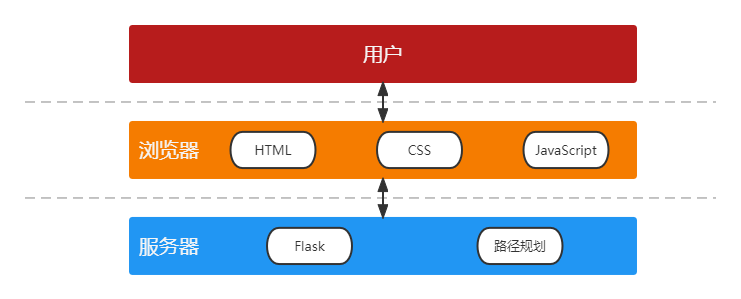
\includegraphics[width = 0.9\textwidth]{fg5_bs}
	\caption{系统设计框架图}
	\label{fg601}
\end{figure}


使用这样的系统框架,可以使得前端界面的展示与后台的路径规划计算相互独立,可以实现高内聚低耦合,降低了今后对于系统的维护成本,实现了前后端分离,提高了工作效率,使得前后端分工更加明确,也能够实现页面的按需加载,可以提高页面交互性能和用户使用体验。

\section{系统成果展示}[en title]
\subsection{使用方法}[en title]
在使用本系统时,用户需要在浏览器中打开本系统的网址。页面左侧的是参数设置模块,右侧是实际区域的地图,用户可以根据需要设置待救援点的位置,无人机基地的位置,无人机的数量、型号、载重和续航里程等信息,确认无误后点击“提交”按钮,即可生成最终的规划路径。
\subsection{页面展示}[en title]
如【占位符】所示,系统界面主要分为2个部分,左侧为相关参数的输入设置,右侧为地图的展示区域。地图中除了实际的地图显示,还使用符号标记了用户设置的兴趣点和无人机基地信息。

而左侧的参数设置区域又可以分为兴趣点参数设置和无人机参数设置两个模块,分别如【占位符】和【占位符】所示:

当用户选择了无人机的救援区域并完成了相关的参数设置后,点击“提交”按钮,前端界面将会把参数和信息通过JSON格式传输至后端,交由其计算最优的无人机飞行路径,再将其传至前端,
这时前端界面便会开始展示无人机的飞行路径,如【占位符】所示:

\section{本章小结}[Brief summary]
本章对无人机紧急救援模拟系统进行了设计与实现,并展示了最终的实现效果。

% 开始写正文之后的部分
\backmatter

%%%% \begin{本科书序} %%%% 这是一个假的环境,本科请用这里的内容

% 结论
% !TEX root = ../main.tex

% 结论
\begin{conclusions}
自然环境的不断变化和无人机等高新技术的发展使得应急救援领域有了新的挑战和新的工具,面对传统运输车辆无法顺利进行任务的复杂环境,无人机成为了一个重要的紧急物资运输工具的选择。而在使用无人机进行紧急救援物资投放时,如何规划高覆盖率的无人机路径成为了一个重要问题。
本文通过对带时间窗的车辆路径规划问题相关文献的研究,在传统VRPTW问题的基础上,考虑了无人机作为运输载具的特殊性,以提升无人机扫描覆盖问题的有效覆盖率为目标,对带时间窗的无人机扫描覆盖问题进行了研究。


本文的主要工作如下:
\begin{itemize}
	\item [(1)] 针对无人机参与的应急救援情况下物资运输问题,建立了无人机紧急救援系统的问题模型。在该模型中,将待救援地点统称为兴趣点,所有无人机从基地出发,按照规划路径对兴趣点进行覆盖,最后返回无人机基地,完成任务。
 	\item [(2)] 提出了带载重的贪婪成本选择算法和带自交的遗传算法来求解问题模型。为了提高算法性能,在原算法基础上进行了相应的改进,以帮助寻求问题的最优解。同时进行了仿真实验,评估了算法的性能。实验结果表明,带载重的贪婪成本选择算法和带自交的遗传算法均能有效解决这一问题模型,且带自交的遗传算法的有效覆盖率$R_e$更高,无人机的飞行成本更低。
\end{itemize}


本文在一定程度上实现了开题时的设定目标,但在后续的研究中,我们发现本文的研究成果还存在以下问题:
\begin{itemize}
	\item [(1)] 本文在研究救援物资时忽略了其体积。在现实场景中,不同物资的规格相差较大,可能会影响无人机的运输效率,该部分还有待未来的进一步研究。
 	\item [(2)] 本文在研究无人机飞行过程时,认为无人机会以恒定速度和恒定续航里程飞行。但是在现实场景中,无人机的飞行速度和续航里程会受自然环境、载重和航向等多重因素的共同影响,在下一步研究中希望能分析无人机飞行速度和续航时间与上述因素之间的关系,而非完全理想化使用固定的速度和续航里程。
\end{itemize}

\end{conclusions}

% 参考文献
\bibliographystyle{hitszthesis}
\bibliography{reference}

% 授权
\authorization

% 授权页为扫描的PDF文件(scan.pdf),与上面的命令互斥
% \authorization[scan.pdf]

% 致谢
% !TEX root = ../main.tex

% 致谢
\begin{acknowledgements}
四年的大学生活时光已经快要结束了,在这四年的学习中,我不仅学习到了计算机科学与技术专业相关的基础知识,更重要的是我认识了自主学习的重要性和必要性,以及为人处世的能力。
感谢父母和家人对我大学四年学习和生活的支持,感谢哈尔滨工业大学(深圳)和计算机科学与技术学院的各位老师大学四年来对我的辛勤培养和教育,各位老师不仅传授给我学科知识,更教会了我做人的道理。


在做毕业设计的这段时间,非常感谢指导老师堵宏伟老师提供的帮助。堵宏伟老师专业知识渊博,治学态度严谨,工作作风一丝不苟,师德崇高,对我今后的工作和学习有着深远的影响。堵宏伟老师在科研和教学
之余,指导学生毕业设计的任务非常繁重,但他依然对于我的毕业设计耐心指导。我还要感谢王慧珍师姐在毕业设计期间提供的宝贵帮助和建议。感谢哈工大(深圳)\LaTeX{}论文模板\hitszthesis\ 
为本人论文撰写过程中提供的便利。


最后感谢参与评审和答辩的各位老师和专家,感谢各位在百忙之中花费时间审阅本人的论文,非常感谢您的宝贵意见。
\end{acknowledgements}


% 附录
% 设置附录部分只包含页眉
% \SetAppendixWithOnlyHeadings
% 设置附录部分页码从1开始编号的命令在<back/appendix01.tex>里
%\begin{appendix}
%  % !TEX root = ../main.tex

% 附录1
\chapter{外文资料翻译}
% 设置附录页码从1开始编号
% \SetPageNumberingFromOne

\title{英文资料的中文标题}

{\heiti 摘要:} 本章为外文资料翻译内容。如果有摘要可以直接写上来,这部分好像没有
明确的规定。

\section{单目标规划}
北冥有鱼,其名为鲲。鲲之大,不知其几千里也。化而为鸟,其名为鹏。鹏之背,不知其几
千里也。怒而飞,其翼若垂天之云。是鸟也,海运则将徙于南冥。南冥者,天池也。
\begin{equation}\tag*{(123)}
 p(y|\mathbf{x}) = \frac{p(\mathbf{x},y)}{p(\mathbf{x})}=
\frac{p(\mathbf{x}|y)p(y)}{p(\mathbf{x})}
\end{equation}

吾生也有涯,而知也无涯。以有涯随无涯,殆已!已而为知者,殆而已矣!为善无近名,为
恶无近刑,缘督以为经,可以保身,可以全生,可以养亲,可以尽年。

\subsection{线性规划}
庖丁为文惠君解牛,手之所触,肩之所倚,足之所履,膝之所倚,砉然响然,奏刀騞然,莫
不中音,合于桑林之舞,乃中经首之会。
\begin{table}[ht]
  \centering
  \wuhao
  \caption*{表~1\hskip1em 这是手动编号但不出现在索引中的一个表格例子}
  \label{tab:badtabular3}
  \begin{tabular}[c]{|m{1.5cm}|c|c|c|c|c|c|}\hline
    \multicolumn{2}{|c|}{Network Topology} & \# of nodes &
    \multicolumn{3}{c|}{\# of clients} & Server \\\hline
    GT-ITM & Waxman Transit-Stub & 600 &
    \multirow{2}{2em}{2\%}&
    \multirow{2}{2em}{10\%}&
    \multirow{2}{2em}{50\%}&
    \multirow{2}{1.2in}{Max. Connectivity}\\\cline{1-3}
    \multicolumn{2}{|c|}{Inet-2.1} & 6000 & & & &\\\hline
    & \multicolumn{2}{c|}{ABCDEF} &\multicolumn{4}{c|}{} \\\hline
\end{tabular}
\end{table}

文惠君曰:“嘻,善哉!技盖至此乎?”庖丁释刀对曰:“臣之所好者道也,进乎技矣。始臣之
解牛之时,所见无非全牛者;三年之后,未尝见全牛也;方今之时,臣以神遇而不以目视,
官知止而神欲行。依乎天理,批大郤,导大窾,因其固然。技经肯綮之未尝,而况大坬乎!
良庖岁更刀,割也;族庖月更刀,折也;今臣之刀十九年矣,所解数千牛矣,而刀刃若新发
于硎。彼节者有间而刀刃者无厚,以无厚入有间,恢恢乎其于游刃必有余地矣。是以十九年
而刀刃若新发于硎。虽然,每至于族,吾见其难为,怵然为戒,视为止,行为迟,动刀甚微,
謋然已解,如土委地。提刀而立,为之而四顾,为之踌躇满志,善刀而藏之。”

文惠君曰:“善哉!吾闻庖丁之言,得养生焉。”


\subsection{非线性规划}
孔子与柳下季为友,柳下季之弟名曰盗跖。盗跖从卒九千人,横行天下,侵暴诸侯。穴室枢
户,驱人牛马,取人妇女。贪得忘亲,不顾父母兄弟,不祭先祖。所过之邑,大国守城,小
国入保,万民苦之。孔子谓柳下季曰:“夫为人父者,必能诏其子;为人兄者,必能教其弟。
若父不能诏其子,兄不能教其弟,则无贵父子兄弟之亲矣。今先生,世之才士也,弟为盗
跖,为天下害,而弗能教也,丘窃为先生羞之。丘请为先生往说之。”

柳下季曰:“先生言为人父者必能诏其子,为人兄者必能教其弟,若子不听父之诏,弟不受
兄之教,虽今先生之辩,将奈之何哉?且跖之为人也,心如涌泉,意如飘风,强足以距敌,
辩足以饰非。顺其心则喜,逆其心则怒,易辱人以言。先生必无往。”

孔子不听,颜回为驭,子贡为右,往见盗跖。

\subsection{整数规划}
盗跖乃方休卒徒大山之阳,脍人肝而餔之。孔子下车而前,见谒者曰:“鲁人孔丘,闻将军
高义,敬再拜谒者。”谒者入通。盗跖闻之大怒,目如明星,发上指冠,曰:“此夫鲁国之
巧伪人孔丘非邪?为我告之:尔作言造语,妄称文、武,冠枝木之冠,带死牛之胁,多辞缪
说,不耕而食,不织而衣,摇唇鼓舌,擅生是非,以迷天下之主,使天下学士不反其本,妄
作孝弟,而侥幸于封侯富贵者也。子之罪大极重,疾走归!不然,我将以子肝益昼餔之膳。”
%  % !TEX root = ../main.tex

% 附录2
\chapter{外文资料原文}
\label{cha:engorg}

\title{The title of the English paper}

\textbf{Abstract:} As one of the most widely used techniques in operations
research, \emph{ mathematical programming} is defined as a means of maximizing a
quantity known as \emph{bjective function}, subject to a set of constraints
represented by equations and inequalities. Some known subtopics of mathematical
programming are linear programming, nonlinear programming, multiobjective
programming, goal programming, dynamic programming, and multilevel
programming$^{[1]}$.

It is impossible to cover in a single chapter every concept of mathematical
programming. This chapter introduces only the basic concepts and techniques of
mathematical programming such that readers gain an understanding of them
throughout the book$^{[2,3]}$.


\section{Single-Objective Programming}
The general form of single-objective programming (SOP) is written
as follows,
\begin{equation}\tag*{(123)} % 如果附录中的公式不想让它出现在公式索引中,那就请
                             % 用 \tag*{xxxx}
\left\{\begin{array}{l}
\max \,\,f(x)\\[0.1 cm]
\mbox{subject to:} \\ [0.1 cm]
\qquad g_j(x)\le 0,\quad j=1,2,\cdots,p
\end{array}\right.
\end{equation}
which maximizes a real-valued function $f$ of
$x=(x_1,x_2,\cdots,x_n)$ subject to a set of constraints.

\newtheorem{mpdef}{Definition}[chapter]
\begin{mpdef}
In SOP, we call $x$ a decision vector, and
$x_1,x_2,\cdots,x_n$ decision variables. The function
$f$ is called the objective function. The set
\begin{equation}\tag*{(456)} % 这里同理,其它不再一一指定。
S=\left\{x\in\Re^n\bigm|g_j(x)\le 0,\,j=1,2,\cdots,p\right\}
\end{equation}
is called the feasible set. An element $x$ in $S$ is called a
feasible solution.
\end{mpdef}

\newtheorem{mpdefop}[mpdef]{Definition}
\begin{mpdefop}
A feasible solution $x^*$ is called the optimal
solution of SOP if and only if
\begin{equation}
f(x^*)\ge f(x)
\end{equation}
for any feasible solution $x$.
\end{mpdefop}

One of the outstanding contributions to mathematical programming was known as
the Kuhn-Tucker conditions\ref{eq:ktc}. In order to introduce them, let us give
some definitions. An inequality constraint $g_j(x)\le 0$ is said to be active at
a point $x^*$ if $g_j(x^*)=0$. A point $x^*$ satisfying $g_j(x^*)\le 0$ is said
to be regular if the gradient vectors $\nabla g_j(x)$ of all active constraints
are linearly independent.

Let $x^*$ be a regular point of the constraints of SOP and assume that all the
functions $f(x)$ and $g_j(x),j=1,2,\cdots,p$ are differentiable. If $x^*$ is a
local optimal solution, then there exist Lagrange multipliers
$\lambda_j,j=1,2,\cdots,p$ such that the following Kuhn-Tucker conditions hold,
\begin{equation}
\label{eq:ktc}
\left\{\begin{array}{l}
    \nabla f(x^*)-\sum\limits_{j=1}^p\lambda_j\nabla g_j(x^*)=0\\[0.3cm]
    \lambda_jg_j(x^*)=0,\quad j=1,2,\cdots,p\\[0.2cm]
    \lambda_j\ge 0,\quad j=1,2,\cdots,p.
\end{array}\right.
\end{equation}
If all the functions $f(x)$ and $g_j(x),j=1,2,\cdots,p$ are convex and
differentiable, and the point $x^*$ satisfies the Kuhn-Tucker conditions
(\ref{eq:ktc}), then it has been proved that the point $x^*$ is a global optimal
solution of SOP.

\subsection{Linear Programming}
\label{sec:lp}

If the functions $f(x),g_j(x),j=1,2,\cdots,p$ are all linear, then SOP is called
a {\em linear programming}.

The feasible set of linear is always convex. A point $x$ is called an extreme
point of convex set $S$ if $x\in S$ and $x$ cannot be expressed as a convex
combination of two points in $S$. It has been shown that the optimal solution to
linear programming corresponds to an extreme point of its feasible set provided
that the feasible set $S$ is bounded. This fact is the basis of the {\em simplex
  algorithm} which was developed by Dantzig as a very efficient method for
solving linear programming.
\begin{table}[ht]
  \centering
  \appendixcaption{Table~1\hskip1em This is an example for manually numbered table, which
    would not appear in the list of tables}
  \label{tab:badtabular2}
  \wuhao
  \begin{tabular}[c]{|m{1.5cm}|c|c|c|c|c|c|}\hline
    \multicolumn{2}{|c|}{Network Topology} & \# of nodes &
    \multicolumn{3}{c|}{\# of clients} & Server \\\hline
    GT-ITM & Waxman Transit-Stub & 600 &
    \multirow{2}{2em}{2\%}&
    \multirow{2}{2em}{10\%}&
    \multirow{2}{2em}{50\%}&
    \multirow{2}{1.2in}{Max. Connectivity}\\\cline{1-3}
    \multicolumn{2}{|c|}{Inet-2.1} & 6000 & & & &\\\hline
    & \multicolumn{2}{c|}{ABCDEF} &\multicolumn{4}{c|}{} \\\hline
  \end{tabular}
\end{table}

Roughly speaking, the simplex algorithm examines only the extreme points of the
feasible set, rather than all feasible points. At first, the simplex algorithm
selects an extreme point as the initial point. The successive extreme point is
selected so as to improve the objective function value. The procedure is
repeated until no improvement in objective function value can be made. The last
extreme point is the optimal solution.

% 附录算法请用这个新环境 <algorithmen>
\begin{algorithmen}
  \wuhao
  \DontPrintSemicolon
  \KwData{$G=(X,U)$ such that $G^{tc}$ is an order.}
  \KwResult{$G’=(X,V)$ with $V\subseteq U$ such that $G’^{tc}$ is an interval order.}
  \caption{\textsc{Fast}SLAM}
\end{algorithmen}

\subsection{Nonlinear Programming}

If at least one of the functions $f(x),g_j(x),j=1,2,\cdots,p$ is nonlinear, then
SOP is called a {\em nonlinear programming}.

A large number of classical optimization methods have been developed to treat
special-structural nonlinear programming based on the mathematical theory
concerned with analyzing the structure of problems.

Now we consider a nonlinear programming which is confronted solely with
maximizing a real-valued function with domain $\Re^n$.  Whether derivatives are
available or not, the usual strategy is first to select a point in $\Re^n$ which
is thought to be the most likely place where the maximum exists. If there is no
information available on which to base such a selection, a point is chosen at
random. From this first point an attempt is made to construct a sequence of
points, each of which yields an improved objective function value over its
predecessor. The next point to be added to the sequence is chosen by analyzing
the behavior of the function at the previous points. This construction continues
until some termination criterion is met. Methods based upon this strategy are
called {\em ascent methods}, which can be classified as {\em direct methods},
{\em gradient methods}, and {\em Hessian methods} according to the information
about the behavior of objective function $f$. Direct methods require only that
the function can be evaluated at each point. Gradient methods require the
evaluation of first derivatives of $f$. Hessian methods require the evaluation
of second derivatives. In fact, there is no superior method for all
problems. The efficiency of a method is very much dependent upon the objective
function.

\subsection{Integer Programming}

{\em Integer programming} is a special mathematical programming in which all of
the variables are assumed to be only integer values. When there are not only
integer variables but also conventional continuous variables, we call it {\em
  mixed integer programming}. If all the variables are assumed either 0 or 1,
then the problem is termed a {\em zero-one programming}. Although integer
programming can be solved by an {\em exhaustive enumeration} theoretically, it
is impractical to solve realistically sized integer programming problems. The
most successful algorithm so far found to solve integer programming is called
the {\em branch-and-bound enumeration} developed by Balas (1965) and Dakin
(1965). The other technique to integer programming is the {\em cutting plane
  method} developed by Gomory (1959).

\hfill\textit{Uncertain Programming\/}\quad(\textsl{BaoDing Liu, 2006.2})

\section*{References}
\noindent{\itshape NOTE: These references are only for demonstration. They are
  not real citations in the original text.}

\begin{translationbib}
\item Donald E. Knuth. The \TeX book. Addison-Wesley, 1984. ISBN: 0-201-13448-9
\item Paul W. Abrahams, Karl Berry and Kathryn A. Hargreaves. \TeX\ for the
  Impatient. Addison-Wesley, 1990. ISBN: 0-201-51375-7
\item David Salomon. The advanced \TeX book.  New York : Springer, 1995. ISBN:0-387-94556-3
\end{translationbib}

%  % !TEX root = ../main.tex

% 附录3
\chapter{其它附录}

其他的附录如数据、代码等,可以放在这里。

%\end{appendix}

%%%% \end{本科书序}


%%%% \begin{硕博书序} %%%% 这是一个假的环境,硕、博请用这里的内容

% % 结论
% % !TEX root = ../main.tex

% 结论
\begin{conclusions}
自然环境的不断变化和无人机等高新技术的发展使得应急救援领域有了新的挑战和新的工具,面对传统运输车辆无法顺利进行任务的复杂环境,无人机成为了一个重要的紧急物资运输工具的选择。而在使用无人机进行紧急救援物资投放时,如何规划高覆盖率的无人机路径成为了一个重要问题。
本文通过对带时间窗的车辆路径规划问题相关文献的研究,在传统VRPTW问题的基础上,考虑了无人机作为运输载具的特殊性,以提升无人机扫描覆盖问题的有效覆盖率为目标,对带时间窗的无人机扫描覆盖问题进行了研究。


本文的主要工作如下:
\begin{itemize}
	\item [(1)] 针对无人机参与的应急救援情况下物资运输问题,建立了无人机紧急救援系统的问题模型。在该模型中,将待救援地点统称为兴趣点,所有无人机从基地出发,按照规划路径对兴趣点进行覆盖,最后返回无人机基地,完成任务。
 	\item [(2)] 提出了带载重的贪婪成本选择算法和带自交的遗传算法来求解问题模型。为了提高算法性能,在原算法基础上进行了相应的改进,以帮助寻求问题的最优解。同时进行了仿真实验,评估了算法的性能。实验结果表明,带载重的贪婪成本选择算法和带自交的遗传算法均能有效解决这一问题模型,且带自交的遗传算法的有效覆盖率$R_e$更高,无人机的飞行成本更低。
\end{itemize}


本文在一定程度上实现了开题时的设定目标,但在后续的研究中,我们发现本文的研究成果还存在以下问题:
\begin{itemize}
	\item [(1)] 本文在研究救援物资时忽略了其体积。在现实场景中,不同物资的规格相差较大,可能会影响无人机的运输效率,该部分还有待未来的进一步研究。
 	\item [(2)] 本文在研究无人机飞行过程时,认为无人机会以恒定速度和恒定续航里程飞行。但是在现实场景中,无人机的飞行速度和续航里程会受自然环境、载重和航向等多重因素的共同影响,在下一步研究中希望能分析无人机飞行速度和续航时间与上述因素之间的关系,而非完全理想化使用固定的速度和续航里程。
\end{itemize}

\end{conclusions}

% % 参考文献
% \bibliographystyle{hitszthesis}
% \bibliography{reference}

% % 附录
% \begin{appendix}
%   % !TEX root = ../main.tex

% 附录A
\chapter{带章节的附录}[Full Appendix]

完整的附录内容,包含章节,公式,图表等。

\section{附录节的内容}[Section in Appendix]

这是附录的节的内容。

附录中\figref{fig:appA}:
\begin{figure}[htbp]
\centering
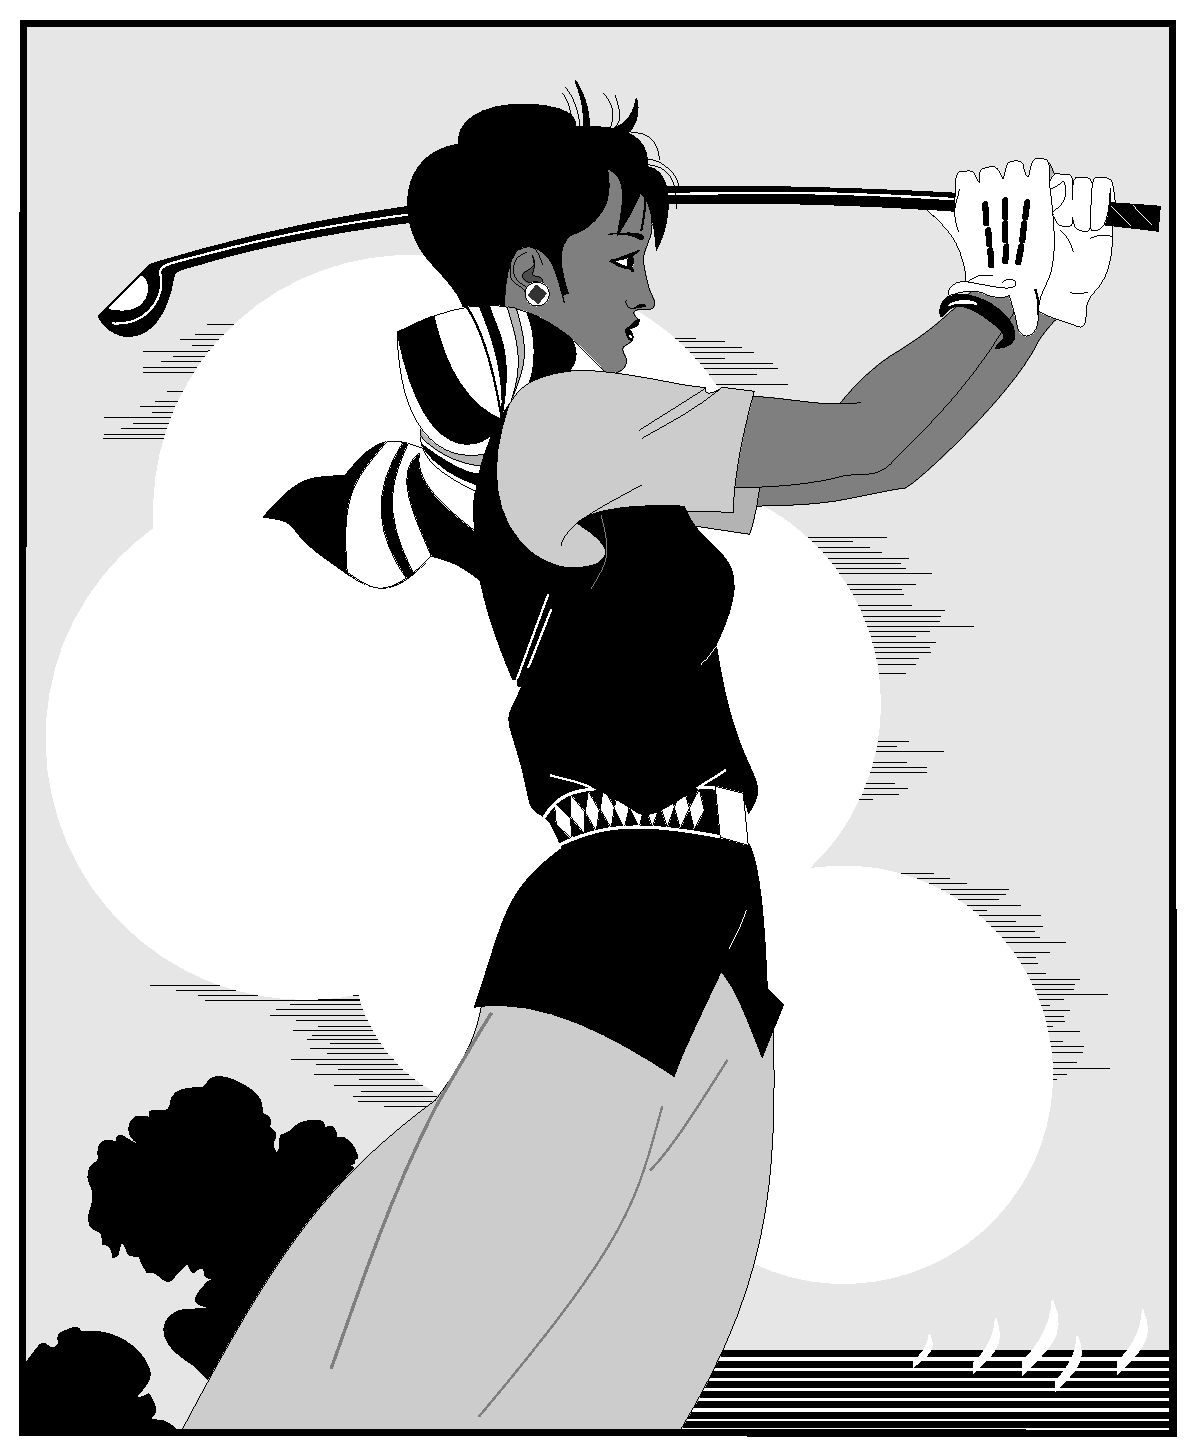
\includegraphics[width = 0.4\textwidth]{golfer}
%\bicaption[golfer5]{}{\xiaosi[0]打高尔夫球的人}{Fig.$\!$}{The person playing golf}\vspace{-1em}
\caption{\xiaosi[0]打高尔夫球的人}
\label{fig:appA}
\end{figure}

附录中\equref{eq:appA}:
\begin{align}
a & = b \times c \\
E & = m c^2
\label{eq:appA}
\end{align}

%   % !TEX root = ../main.tex

% 附录B
\chapter{这个星球上最好的免费Linux软件列表}[List of the Best Linux Software in our Planet]
\section{系统}

\href{http://fvwm.org/}{FVWM 自从上世纪诞生以来,此星球最强大的窗口管理器。}
推荐基于FVWM的桌面设计hifvwm:\href{https://github.com/dustincys/hifvwm}{https://github.com/dustincys/hifvwm}。

\subsection{hifvwm的优点}

\begin{enumerate}
	\item 即使打开上百个窗口也不会“蒙圈”。计算机性能越来越强大,窗口任务的管理必须要升级到打怪兽级别。
	\item 自动同步Bing搜索主页的壁纸。每次电脑开机,午夜零点自动更新,用户
		也可以手动更新,从此审美再也不疲劳。
	\item 切换窗口自动聚焦到最上面的窗口。使用键盘快捷键切换窗口时候,减少
		操作过程,自动聚焦到目标窗口。这一特性是虚拟窗口必须的人性化设
		计。
	\item 类似window右下角的功能的最小化窗口来显示桌面的功能此处类似
		win7/win10,实现在一个桌面之内操作多个任务。
	\item 任务栏结合标题栏。采用任务栏和标题栏结合,节省空间。
	\item 同类窗口切换。可以在同类窗口之内类似alt-tab的方式切换。
	\item ……
\end{enumerate}

\section{其他}

\href{https://orgmode.org/}{orgmode,最强大的笔记系统,从来没有之一。}

\href{https://www.jianguoyun.com/}{坚果云,国内一款支持WebDav的云盘系统,国内真正的云盘没有之一。}

\section{vim}
实现中英文每一句一行,以及实现每一句折叠断行的简单正则式,tex源码更加乖乖。
\begin{lstlisting}
vnoremap <leader>fae J:s/[.!?]\zs\s\+/\="\r".matchstr(getline('.'), '^\s*')/g<CR>
vnoremap <leader>fac J:s/[。!?]/\=submatch(0)."\n".matchstr(getline('.'), '^\s*')/g<CR>
vnoremap <leader>fle :!fmt -80 -s<CR>
\end{lstlisting}

% \end{appendix}

% % 发表文章
% % !TEX root = ../main.tex

% 发表论文、专利、获奖情况
\begin{publication}
  \noindent\songti\textbf{(一)发表的学术论文}
  \begin{publist}
    \item	XXX,XXX. Static Oxidation Model of Al-Mg/C Dissipation Thermal Protection Materials[J]. Rare Metal Materials and Engineering,2010,39(Suppl. 1):520-524.(SCI~收录,IDS号为~669JS,IF=0.16)
    \item XXX,XXX. 精密超声振动切削单晶铜的计算机仿真研究[J]. 系统仿真学报,2007,19(4):738-741,753.(EI~收录号:20071310514841)
    \item XXX,XXX. 局部多孔质气体静压轴向轴承静态特性的数值求解[J]. 摩擦学学报,2007(1):68-72.(EI~收录号:20071510544816)
    \item XXX,XXX. 硬脆光学晶体材料超精密切削理论研究综述[J]. 机械工程学报,2003,39(8):15-22.(EI~收录号:2004088028875)
    \item XXX,XXX. 基于遗传算法的超精密切削加工表面粗糙度预测模型的参数辨识以及切削参数优化[J]. 机械工程学报,2005,41(11):158-162.(EI~收录号:2006039650087)
    \item XXX,XXX. Discrete Sliding Mode Cintrok with Fuzzy Adaptive Reaching Law on 6-PEES Parallel Robot[C]. Intelligent System Design and Applications,Jinan,2006:649-652.(EI~收录号:20073210746529)
  \end{publist}

  \noindent\songti\textbf{(二)申请及已获得的专利(无专利时此项不必列出)}
  \begin{publist}
    \item XXX,XXX. 一种温热外敷药制备方案:中国,88105607.3[P]. 1989-07-26.
  \end{publist}

  \noindent\songti\textbf{(三)参与的科研项目及获奖情况}
  \begin{publist}
    \item	XXX,XXX. XX~气体静压轴承技术研究,XX~省自然科学基金项目.课题编号:XXXX.
    \item XXX,XXX. XX~静载下预应力混凝土房屋结构设计统一理论. 黑江省科学技术二等奖,2007.
  \end{publist}
  %\vfill
  %\hangafter=1\hangindent=2em\noindent
  %\setlength{\parindent}{2em}
\end{publication}


% % 索引
% % % !TEX root = ../main.tex

% 中英文索引
\begin{ceindex}
  \printsubindex*
\end{ceindex}


% % 授权
% \authorization

% % 授权页为扫描的PDF文件(scan.pdf),与上面的命令互斥
% % \authorization[scan.pdf]

% % 致谢
% % !TEX root = ../main.tex

% 致谢
\begin{acknowledgements}
四年的大学生活时光已经快要结束了,在这四年的学习中,我不仅学习到了计算机科学与技术专业相关的基础知识,更重要的是我认识了自主学习的重要性和必要性,以及为人处世的能力。
感谢父母和家人对我大学四年学习和生活的支持,感谢哈尔滨工业大学(深圳)和计算机科学与技术学院的各位老师大学四年来对我的辛勤培养和教育,各位老师不仅传授给我学科知识,更教会了我做人的道理。


在做毕业设计的这段时间,非常感谢指导老师堵宏伟老师提供的帮助。堵宏伟老师专业知识渊博,治学态度严谨,工作作风一丝不苟,师德崇高,对我今后的工作和学习有着深远的影响。堵宏伟老师在科研和教学
之余,指导学生毕业设计的任务非常繁重,但他依然对于我的毕业设计耐心指导。我还要感谢王慧珍师姐在毕业设计期间提供的宝贵帮助和建议。感谢哈工大(深圳)\LaTeX{}论文模板\hitszthesis\ 
为本人论文撰写过程中提供的便利。


最后感谢参与评审和答辩的各位老师和专家,感谢各位在百忙之中花费时间审阅本人的论文,非常感谢您的宝贵意见。
\end{acknowledgements}


% % 个人简介
% % !TEX root = ../main.tex

% 个人简历
\begin{resume}

  XXXX~年~XX~月~XX~日出生于~XXXX。

  XXXX~年~XX~月考入~XX~大学~XX~院(系)XX~专业,XXXX~年~XX~月本科毕业并获得~XX~学学士学位。

  XXXX~年~XX~月------XXXX~年~XX~月在~XX~大学~XX~院(系)XX~学科学习并获得~XX~学硕士学位。

  XXXX~年~XX~月------XXXX~年~XX~月在~XX~大学~XX~院(系)XX~学科学习并获得~XX~学博士学位。

  获奖情况:如获三好学生、优秀团干部、X~奖学金等(不含科研学术获奖)。

  工作经历:

  \songti\textbf{(除全日制硕士生以外,其余学生均应增列此项。个人简历一般应包含教育经历和工作经历。)}

\end{resume}


%%%% \end{硕博书序}


% 结束文档撰写
\end{document}
%%=============================================

% Local Variables:
% TeX-engine: xetex
% End:
